\documentclass{beamer}

\usefonttheme{professionalfonts} % using non standard fonts for beamer
\usefonttheme{serif} % default family is serif

\usepackage{hyperref}

%\usepackage{minted}

\usepackage{animate}

\usepackage{graphicx}

\def\Put(#1,#2)#3{\leavevmode\makebox(0,0){\put(#1,#2){#3}}}

\usepackage{color}

\usepackage{tikz}

\usepackage{amssymb}
\usepackage{amsthm}

\usepackage{enumerate}


\newcommand\blfootnote[1]{%

  \begingroup

  \renewcommand\thefootnote{}\footnote{#1}%

  \addtocounter{footnote}{-1}%

  \endgroup

}

\makeatletter

%%%%%%%%%%%%%%%%%%%%%%%%%%%%%% Textclass specific LaTeX commands.

 % this default might be overridden by plain title style

 \newcommand\makebeamertitle{\frame{\maketitle}}%

 % (ERT) argument for the TOC

 \AtBeginDocument{%

   \let\origtableofcontents=\tableofcontents

   \def\tableofcontents{\@ifnextchar[{\origtableofcontents}{\gobbletableofcontents}}

   \def\gobbletableofcontents#1{\origtableofcontents}

 }

%%%%%%%%%%%%%%%%%%%%%%%%%%%%%% User specified LaTeX commands.

\usetheme{Malmoe}

% or ...

\useoutertheme{infolines}

\addtobeamertemplate{headline}{}{\vskip2pt}

\setbeamertemplate{theorems}[numbered]

\theoremstyle{definition}
\newtheorem{defn}{Definition}[section]

\setbeamercovered{transparent}

% or whatever (possibly just delete it)

\makeatother

\begin{document}
\title[Discussion 8]{CS/MATH 111, Discrete Structures - Fall 2018. \\ Discussion 8 - Graphs}
\author[CS111]{Andres, Sara, Elena}
\institute[Fall'18]{University of California, Riverside}
\makebeamertitle
\newif\iflattersubsect

\AtBeginSection[] {
    \begin{frame}<beamer>
    \frametitle{Outline} 
    \tableofcontents[currentsection]  
    \end{frame}
    \lattersubsectfalse
}

\AtBeginSubsection[] {
    \begin{frame}<beamer>
    \frametitle{Outline} 
    \tableofcontents[currentsubsection]  
    \end{frame}
}

\section{Euler tour}

\begin{frame}{Euler path and tour}
    \begin{defn}
        An \textit{Euler tour} in a graph $G$ is a simple circuit containing \textbf{every edge} of $G$. An \textit{Euler path} in $G$ is a simple path containing every edge of $G$.
    \end{defn}
\end{frame}

\begin{frame}{Euler tour}
    \begin{itemize}
        \item An Euler tour (or Eulerian tour, Euler circuit) traverses each edge of the graph \textbf{exactly once}. 
        \item Graphs that have an Euler tour are called Eulerian. 
      \end{itemize}
\end{frame}

\begin{frame}{Euler tour}
    \begin{theorem}\label{theo:euler1}
        An undirected graph has a closed Euler tour \textit{iff} it is connected and each vertex has an even degree.
    \end{theorem}
   
    \begin{theorem}\label{theo:euler2}
        An undirected graph has an Euler path but not an Euler tour \textit{iff} it has exactly two vertices of odd degree. 
    \end{theorem}
\end{frame}

\begin{frame}{Euler tour}
   \begin{itemize}
        \item So this graph is not Eulerian:
    \end{itemize}
    \centering 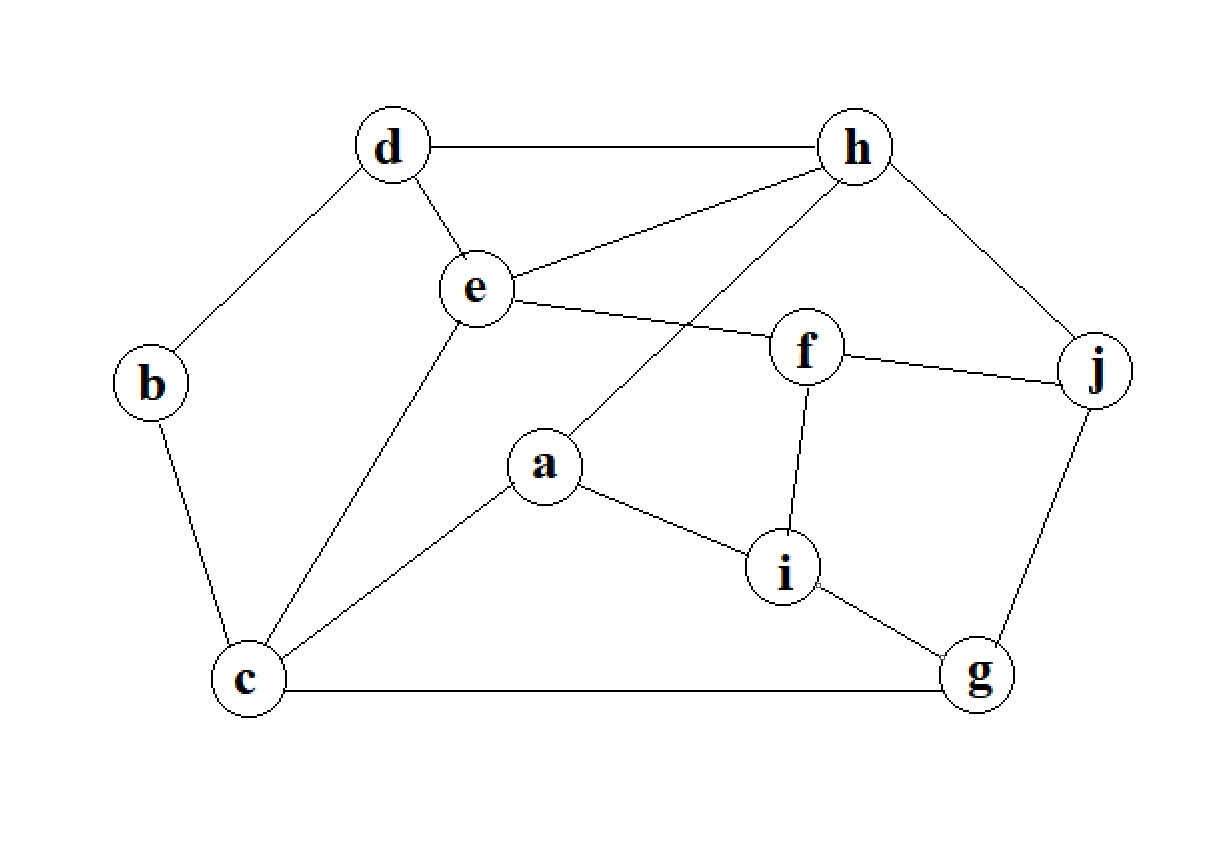
\includegraphics[width=.6\linewidth]{p1.jpg}
\end{frame}

\begin{frame}{Euler tour}
   \begin{itemize}
        \item Mohammed's Scimitars:
    \end{itemize}
    \centering 
    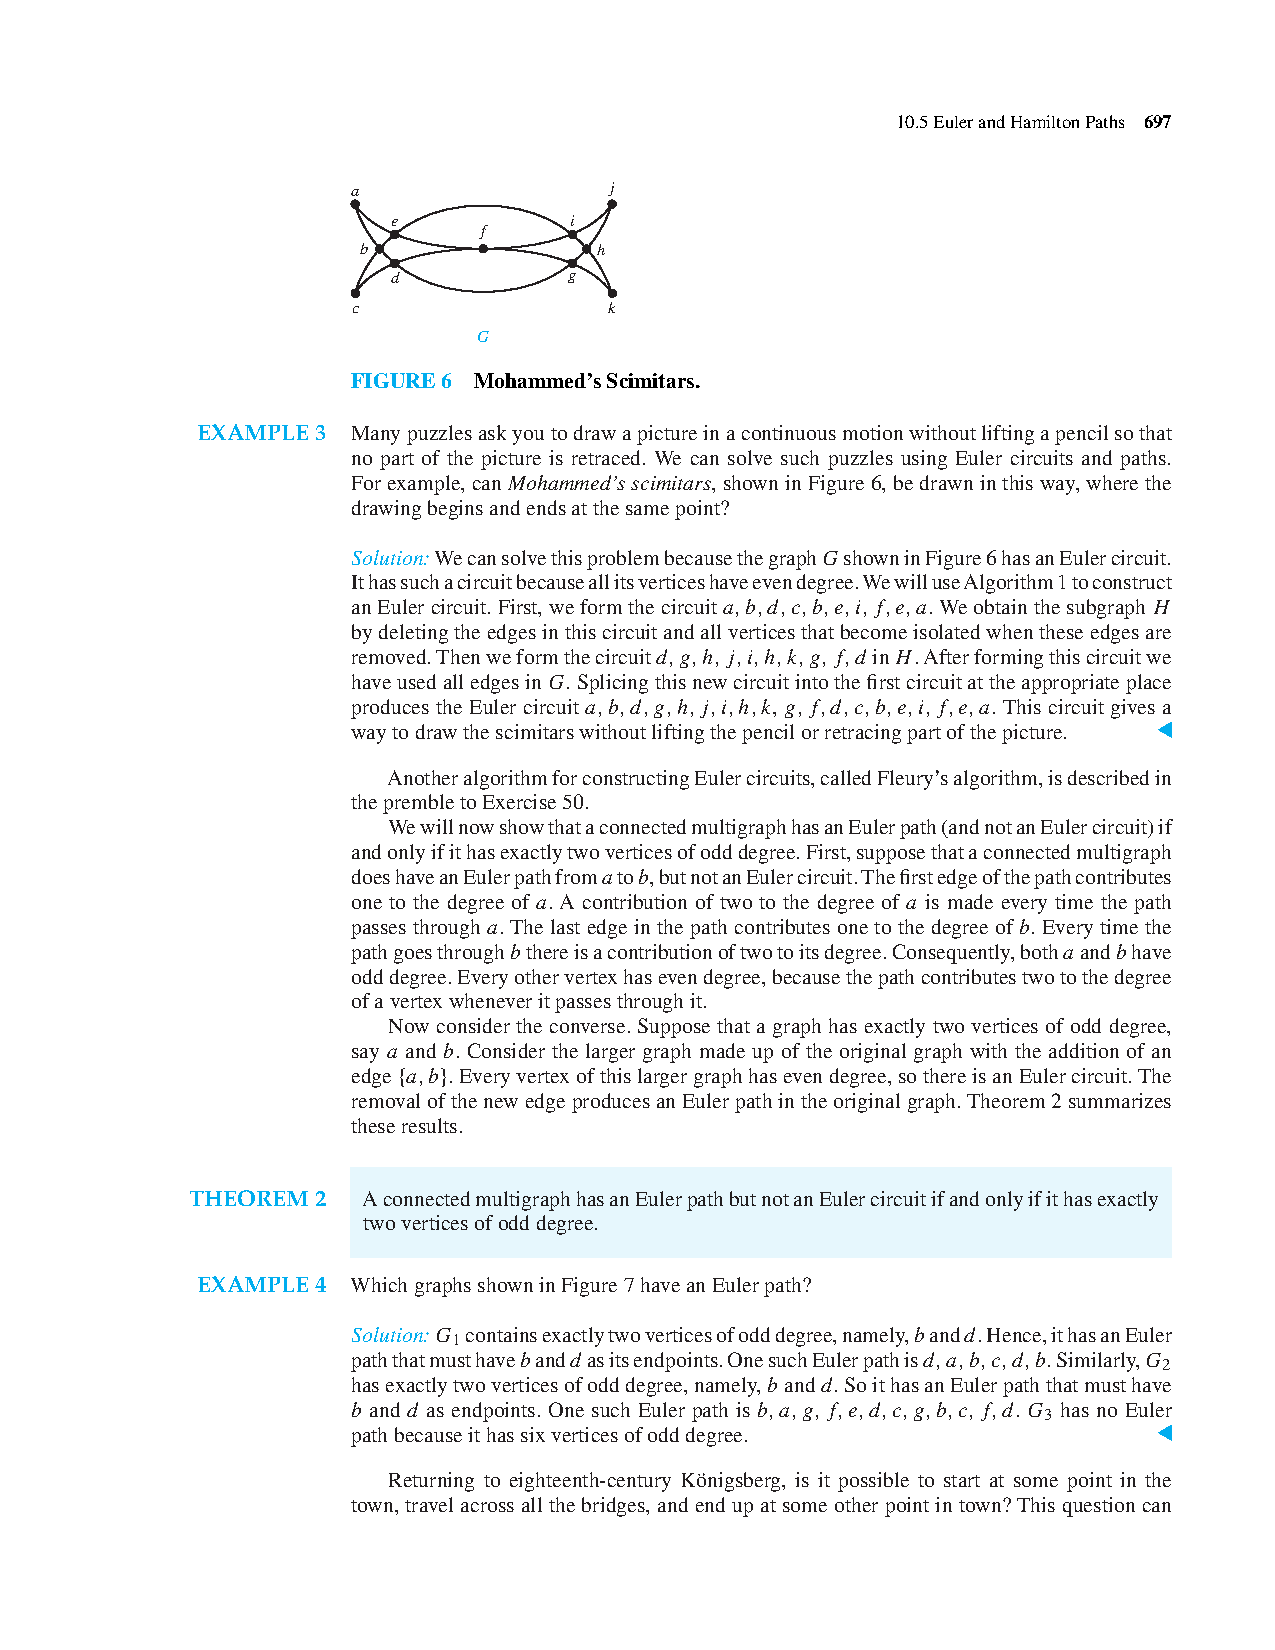
\includegraphics[trim={5cm 22.5cm 10cm 2.5cm},clip,width=.75\linewidth]{p697}
\end{frame}

\begin{frame}{Euler tour}
   \begin{itemize}
        \item Mohammed's Scimitars:
    \end{itemize}
    \centering 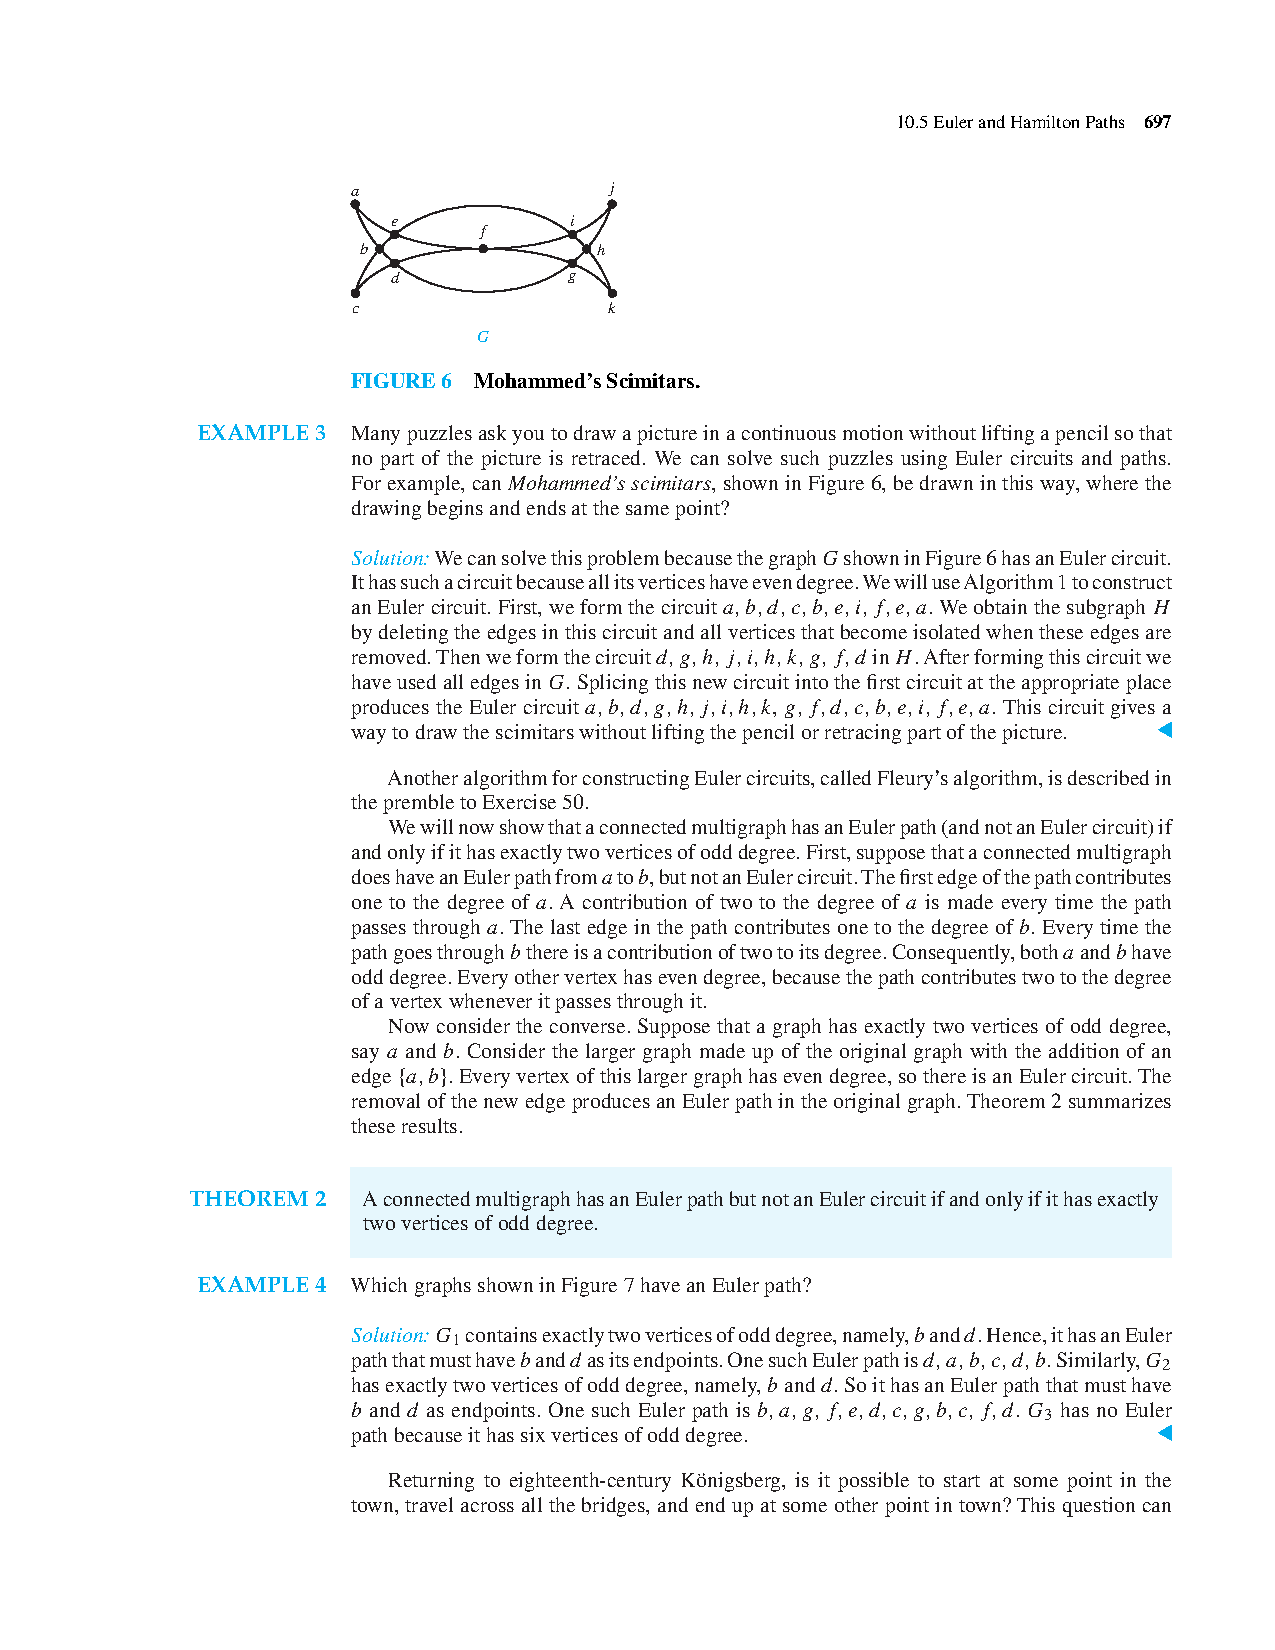
\includegraphics[trim={5cm 22.5cm 10cm 2.5cm},clip,width=.75\linewidth]{p697}
    \\a, b, d, g, h, j, i, h, k, g, f, d, c, b, e, i, f, e, a
\end{frame}

\begin{frame}{Euler tour}
   \begin{itemize}
        \item Determine weather the given graph has an Euler circuit:
    \end{itemize}
    \centering 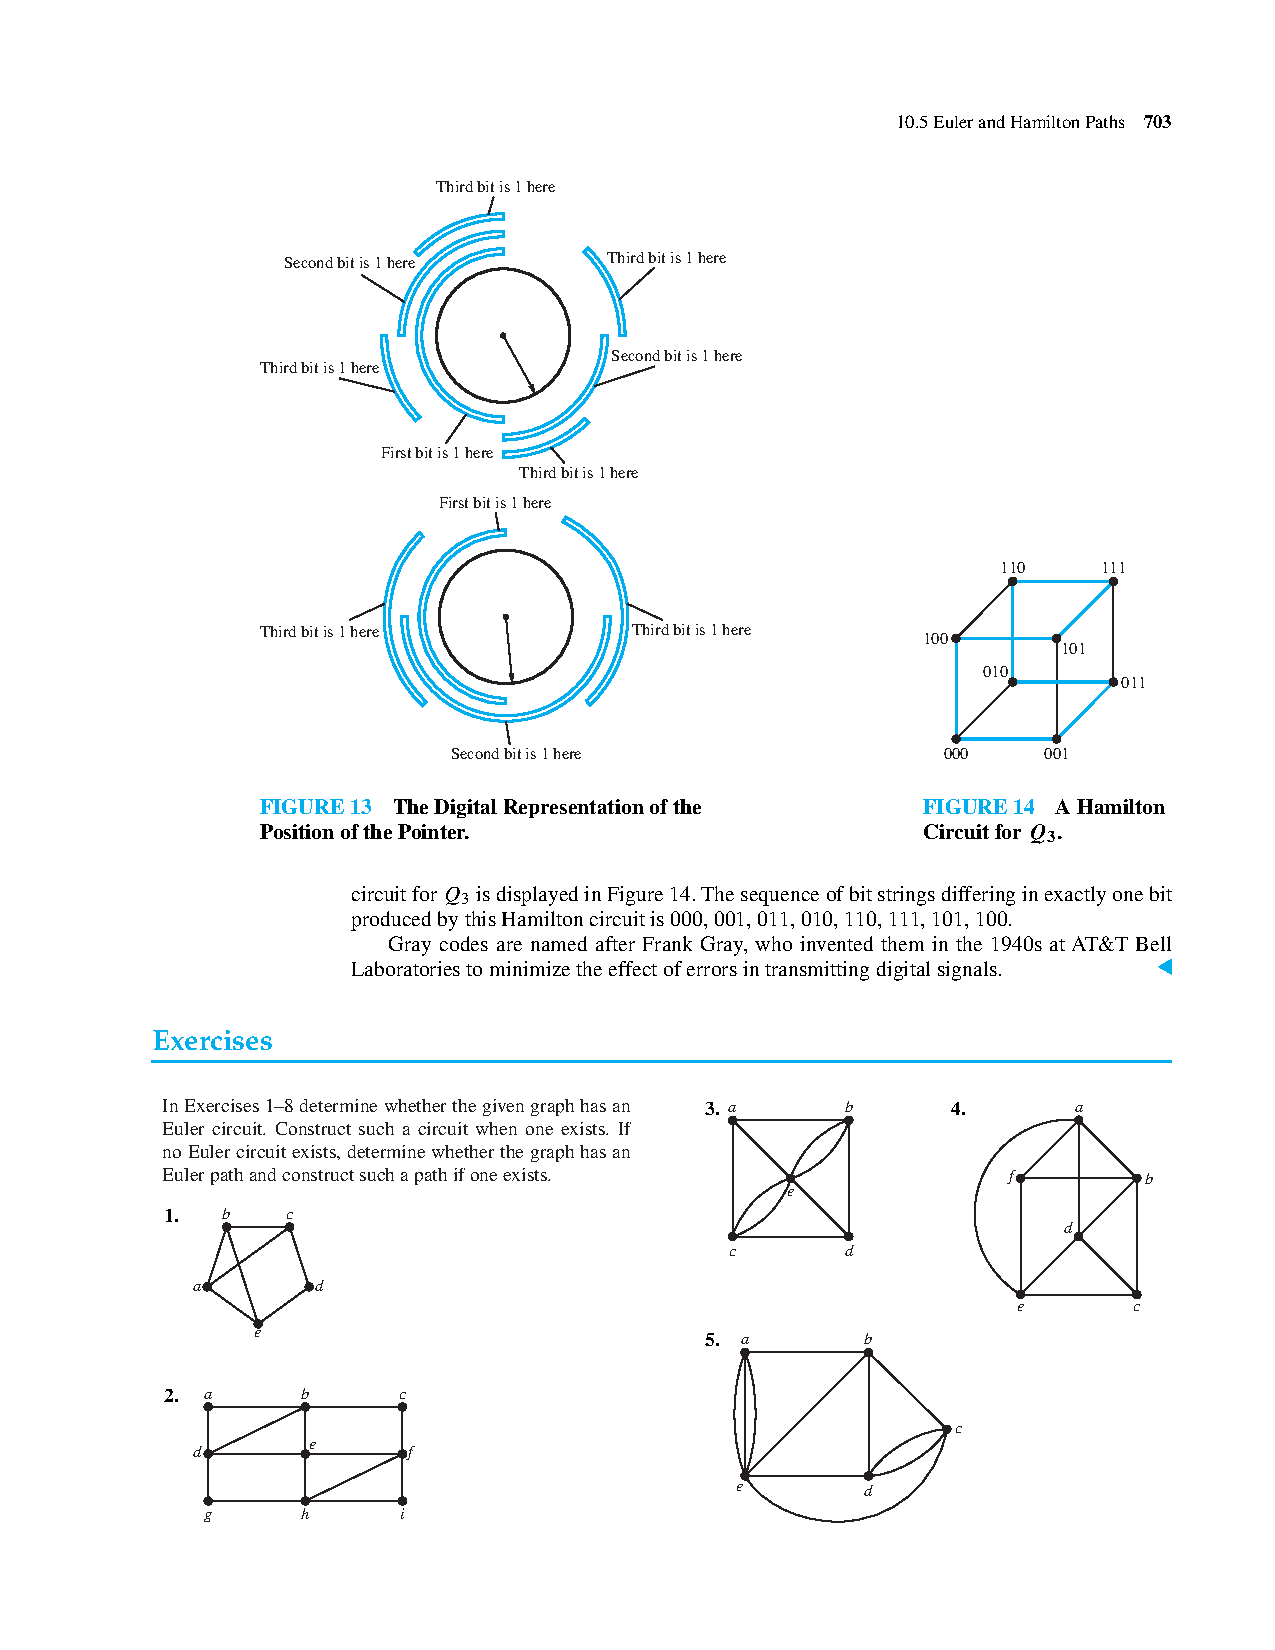
\includegraphics[trim={12.2cm 6cm 6cm 18.2cm},clip,width=.45\linewidth]{p703}
\end{frame}

\begin{frame}{Euler tour}
   \begin{itemize}
        \item Determine weather the given graph has an Euler circuit:
    \end{itemize}
    \centering 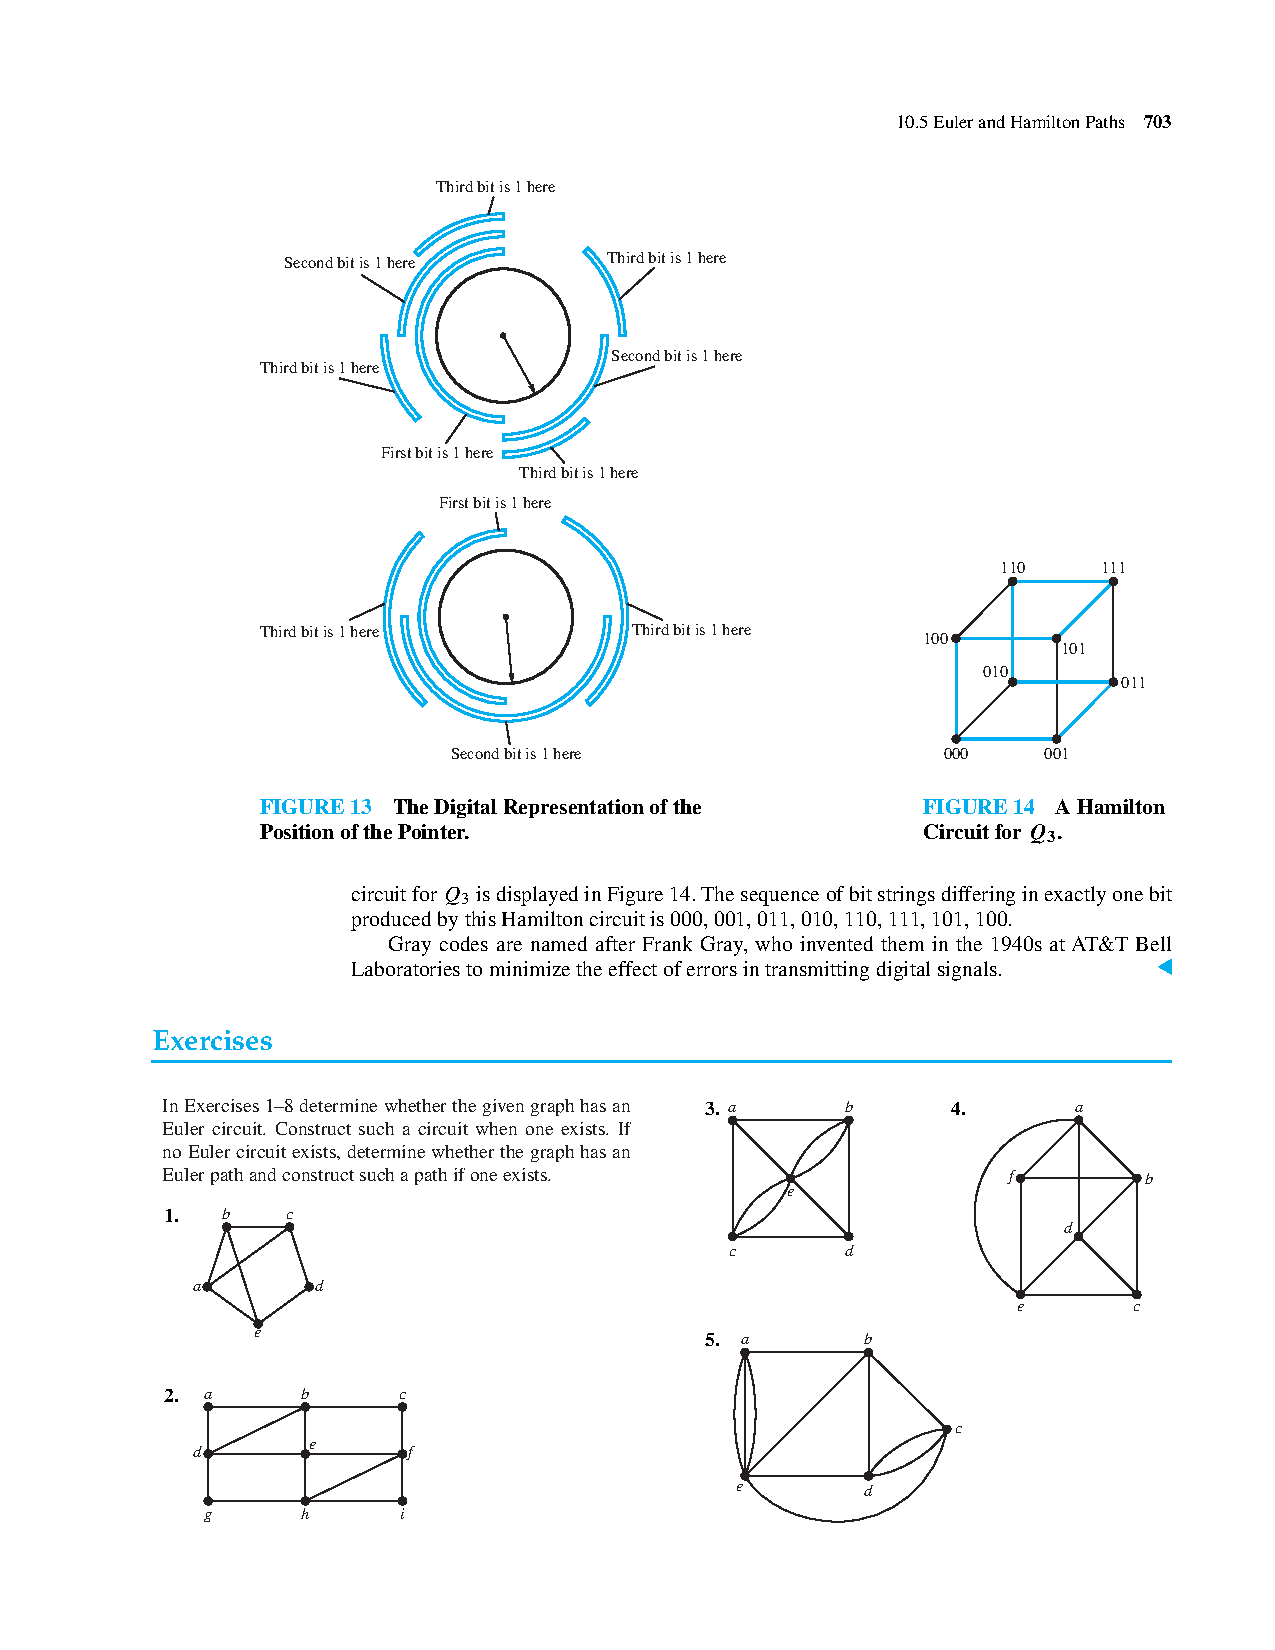
\includegraphics[trim={12.2cm 2cm 5.2cm 22.2cm},clip,width=.45\linewidth]{p703}
\end{frame}

\section{Hamiltonian Cycle}

\begin{frame}{Hamiltonian Cycle}
   \begin{itemize}
        \item Hamiltonian Cycle (or Hamilton circuit) is a graph cycle (i.e., closed loop) through a graph that visits each node exactly once 
    \end{itemize}
\end{frame}

\begin{frame}{Hamiltonian Cycle}
    \begin{theorem}[Dirac's Theorem]\label{theo:dirac}
        If $G$ is a simple graph with $n$ vertices with $n\geq 3$ such that the degree of every vertex in $G$ is at least $\frac{n}{2}$, then $G$ has a Hamilton cycle. 
    \end{theorem}
    \begin{theorem}[Ore's Theorem]\label{theo:ore}
        If G is a simple graph on n vertices, $n\geq 3$, and $d(v)+d(w)\geq n$ whenever v and w are not adjacent, then G has a Hamilton cycle. 
    \end{theorem}
\end{frame}

\begin{frame}{Hamiltonian Cycle}
    \begin{itemize}
        \item The graph does not have Hamiltonian cycle.
    \end{itemize}
    \centering 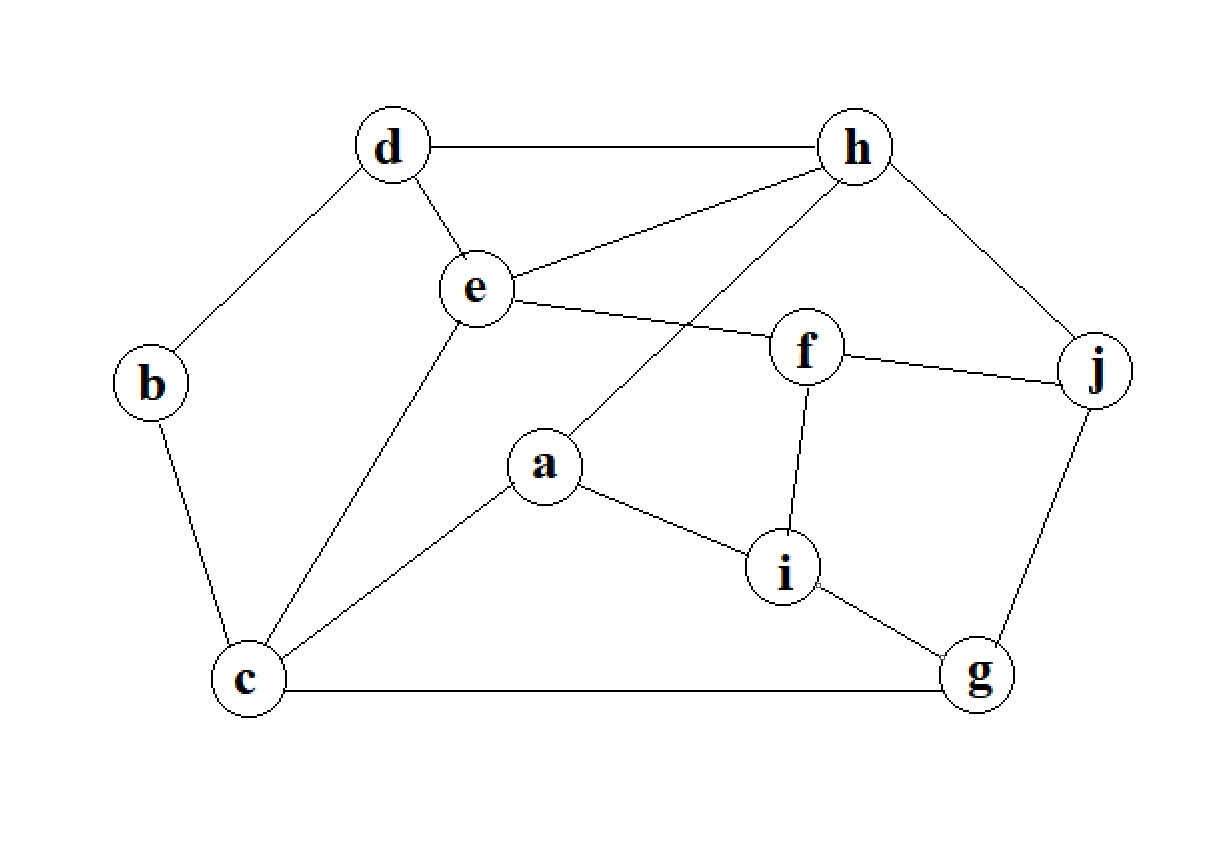
\includegraphics[width=.7\linewidth]{p1.jpg}
\end{frame}

\begin{frame}{Hamiltonian Cycle}
   \begin{itemize}
        \item Determine weather the given graph has a Hamilton circuit:
    \end{itemize}
    \centering 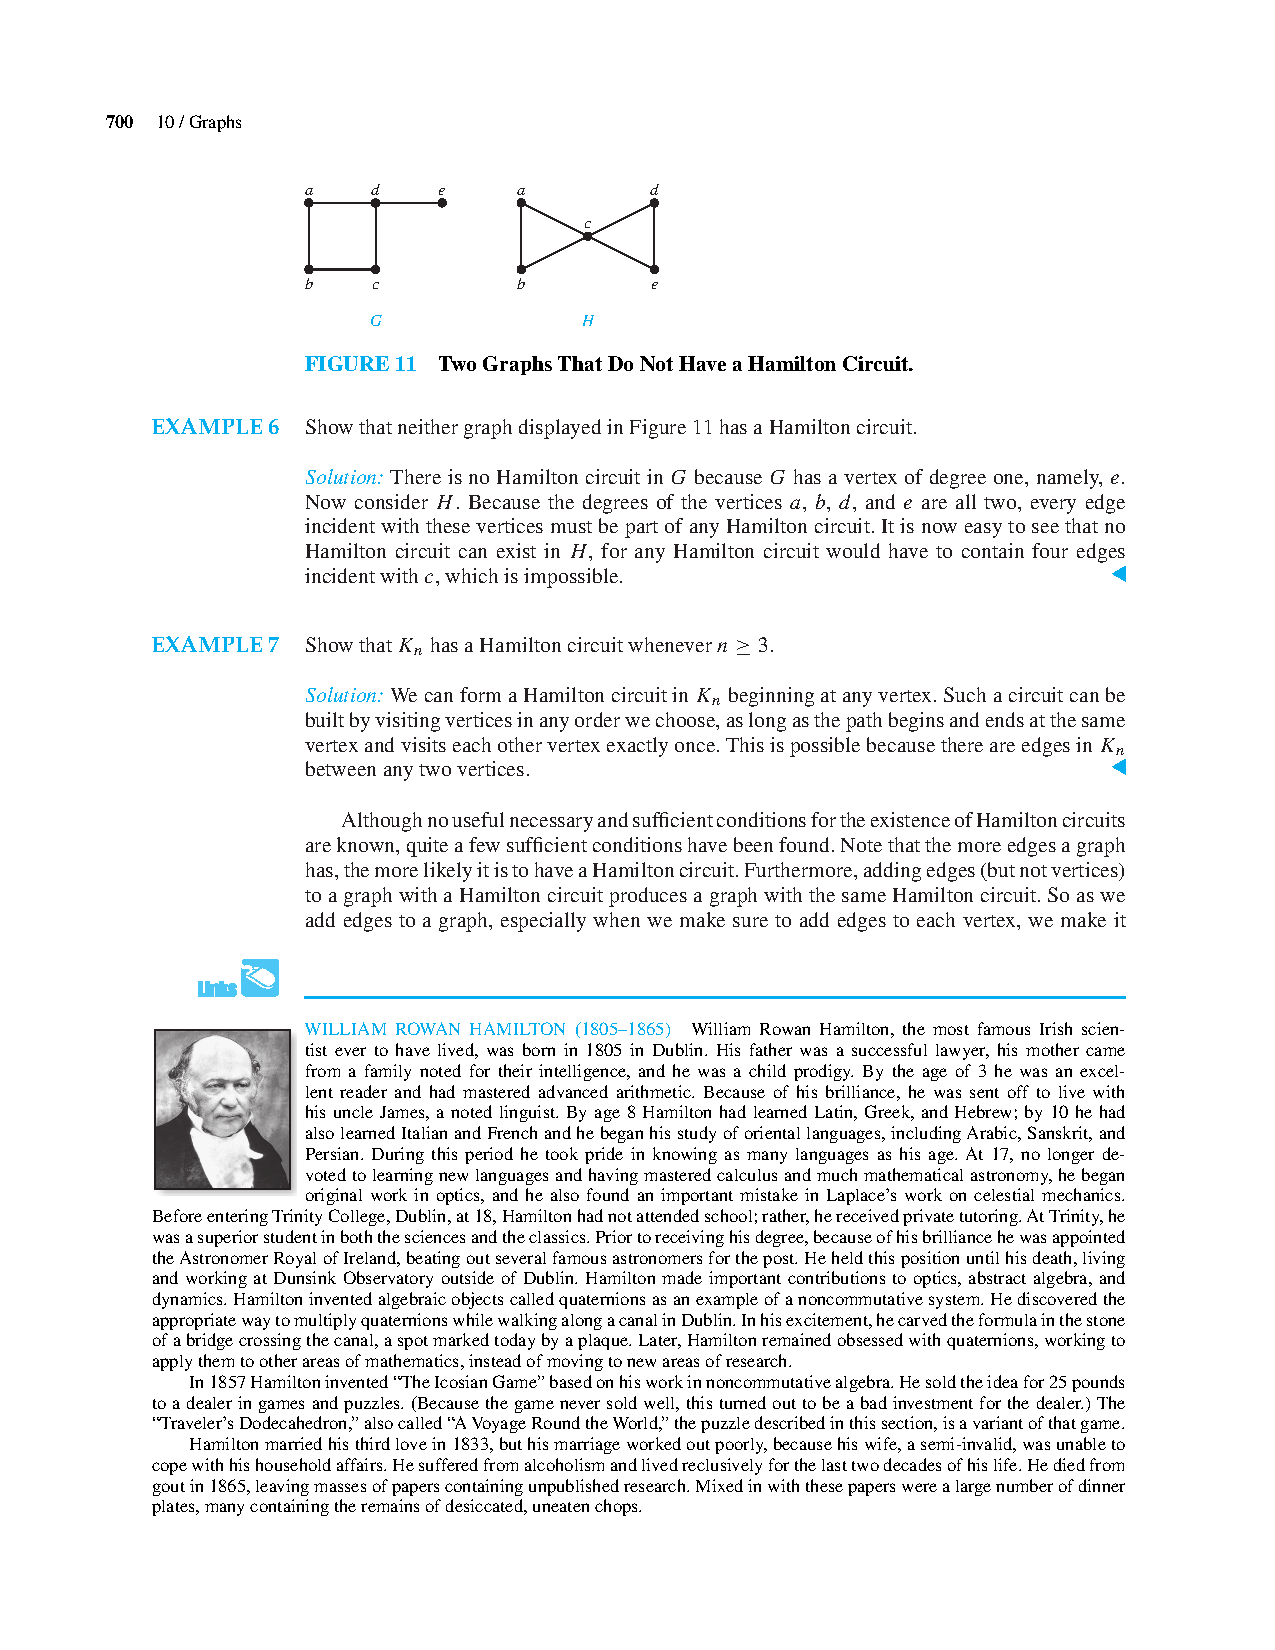
\includegraphics[trim={5cm 23cm 10cm 2cm},clip,width=.8\linewidth]{p700}
\end{frame}

\begin{frame}{Hamiltonian Cycle}
   \begin{itemize}
        \item Determine weather the given graph has a Hamilton circuit:
    \end{itemize}
    \centering 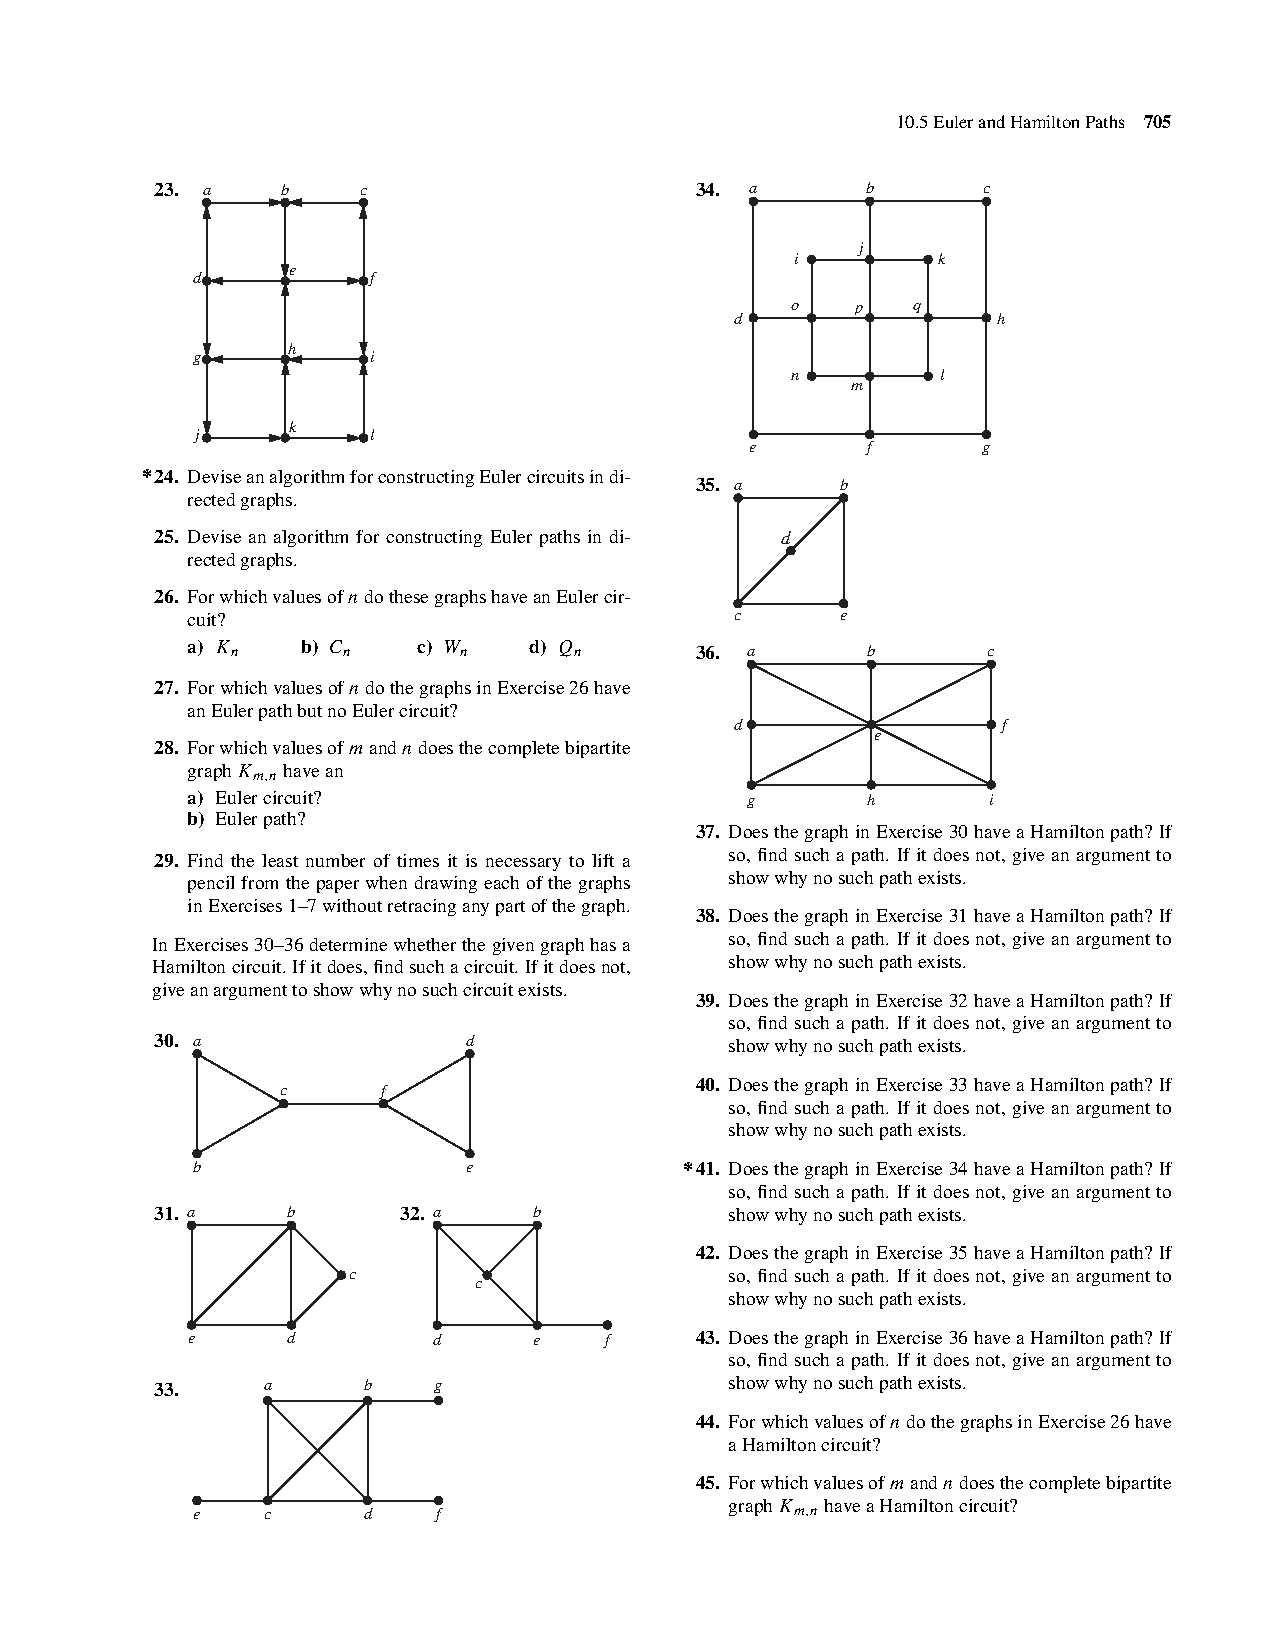
\includegraphics[trim={3.1cm 5cm 15.4cm 20cm},clip,width=.5\linewidth]{p705}
\end{frame}

\begin{frame}{Hamiltonian Cycle}
   \begin{itemize}
        \item Determine weather the given graph has a Hamilton circuit:
    \end{itemize}
    \centering 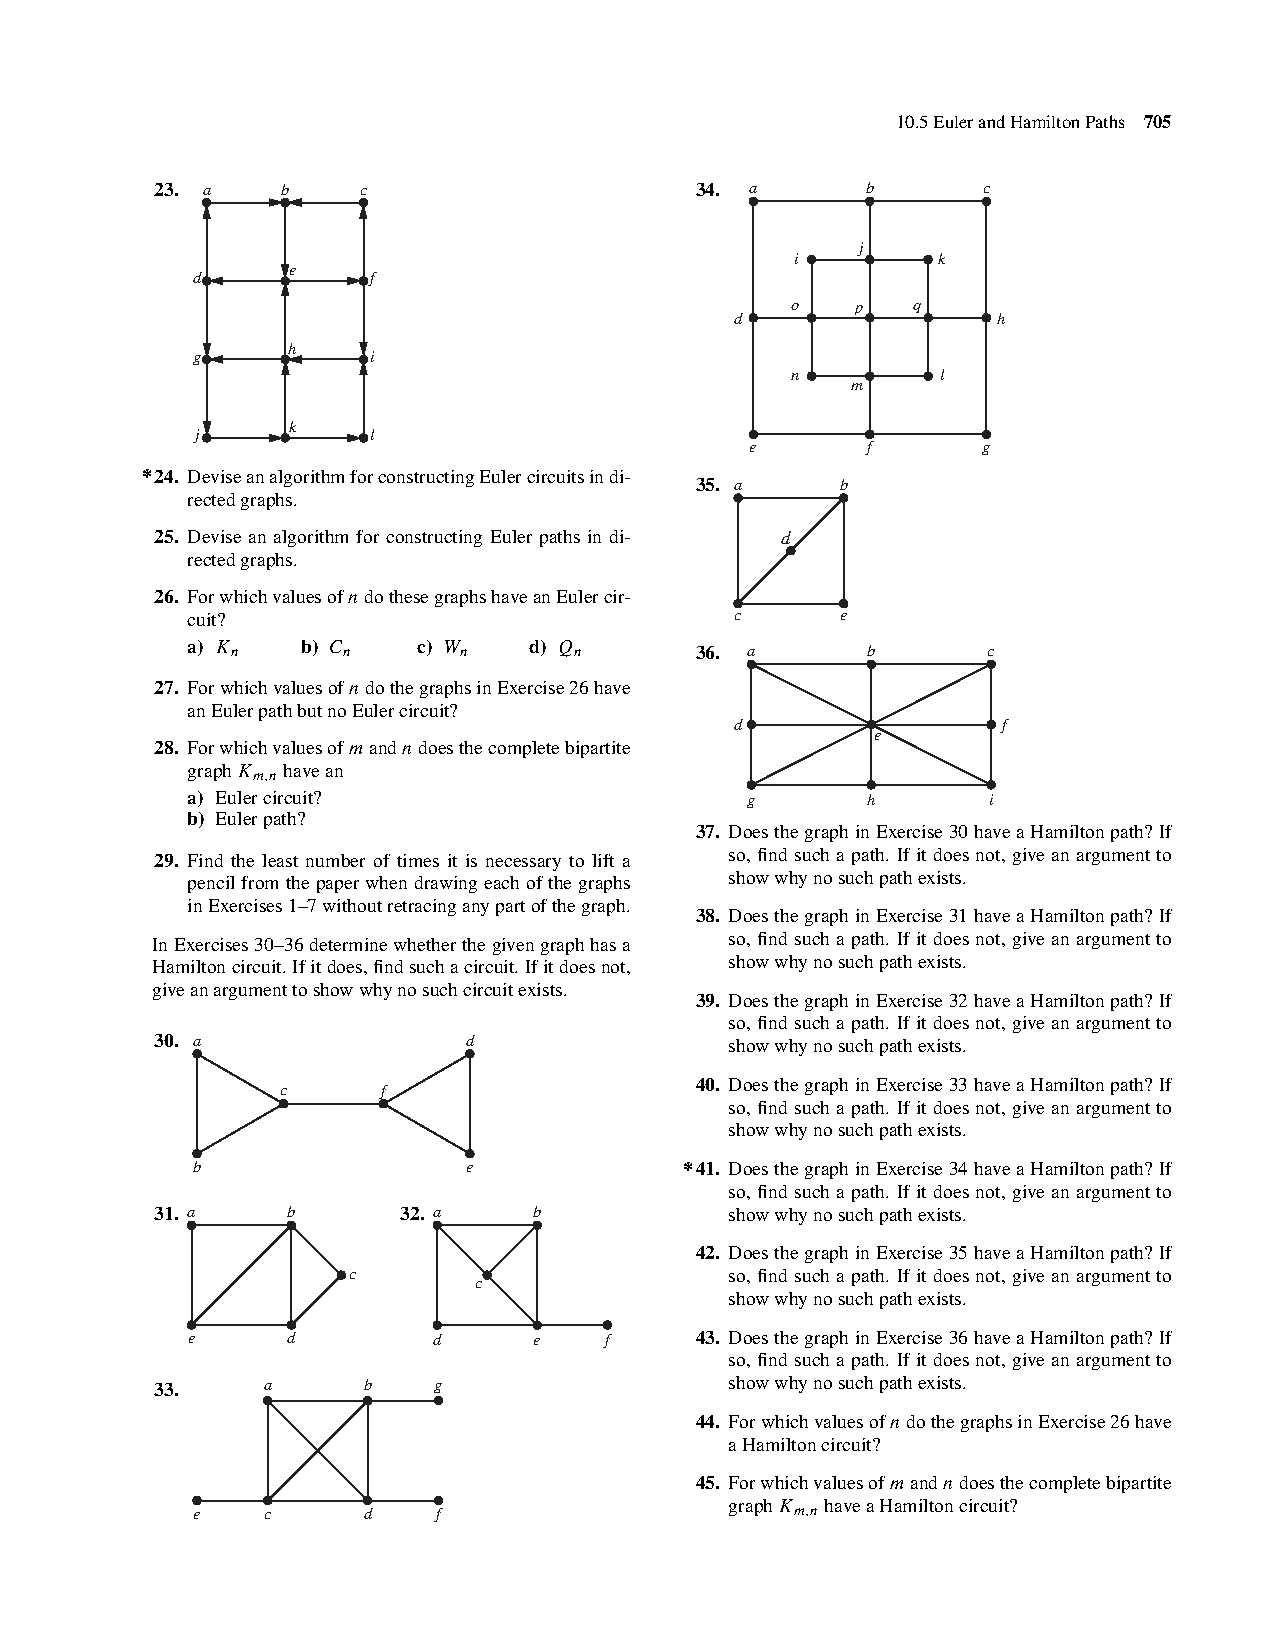
\includegraphics[trim={3.1cm 2cm 14cm 23cm},clip,width=.65\linewidth]{p705}
\end{frame}

\begin{frame}{Hamiltonian Cycle}
   \begin{itemize}
        \item Determine weather the given graph has a Hamilton circuit:
    \end{itemize}
    \centering 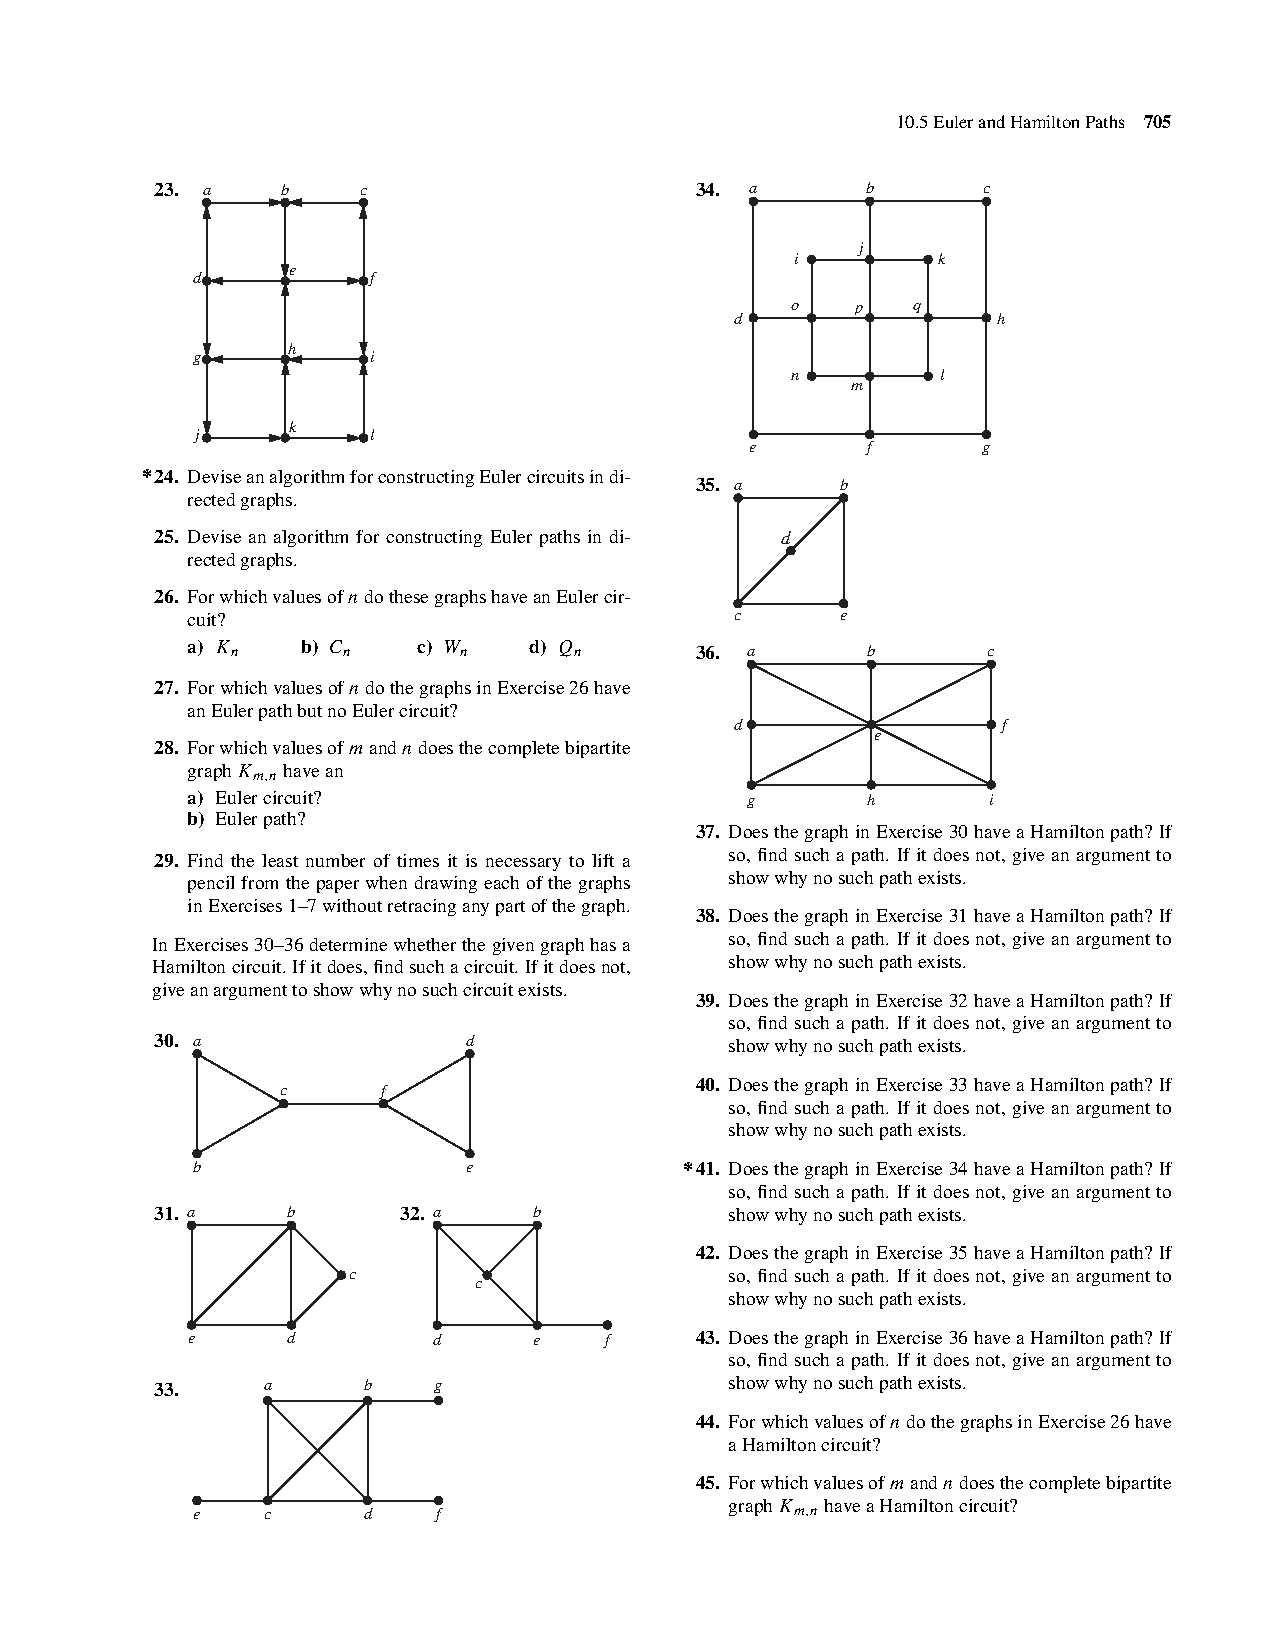
\includegraphics[trim={12.3cm 17.2cm 7cm 8cm},clip,width=.4\linewidth]{p705}
\end{frame}

\begin{frame}{Hamiltonian Cycle}
    \begin{itemize}
        \item For each of these graphs, determine: 
        {\scriptsize
        \begin{enumerate}[(i)]
            \item whether Dirac's theorem can be used to show that the graph has a Hamilton circuit
            \item whether Ore's theorem can be used to show that the graph has a Hamilton circuit
            \item whether the graph has a Hamilton circuit
        \end{enumerate}}
    \end{itemize}
    \centering 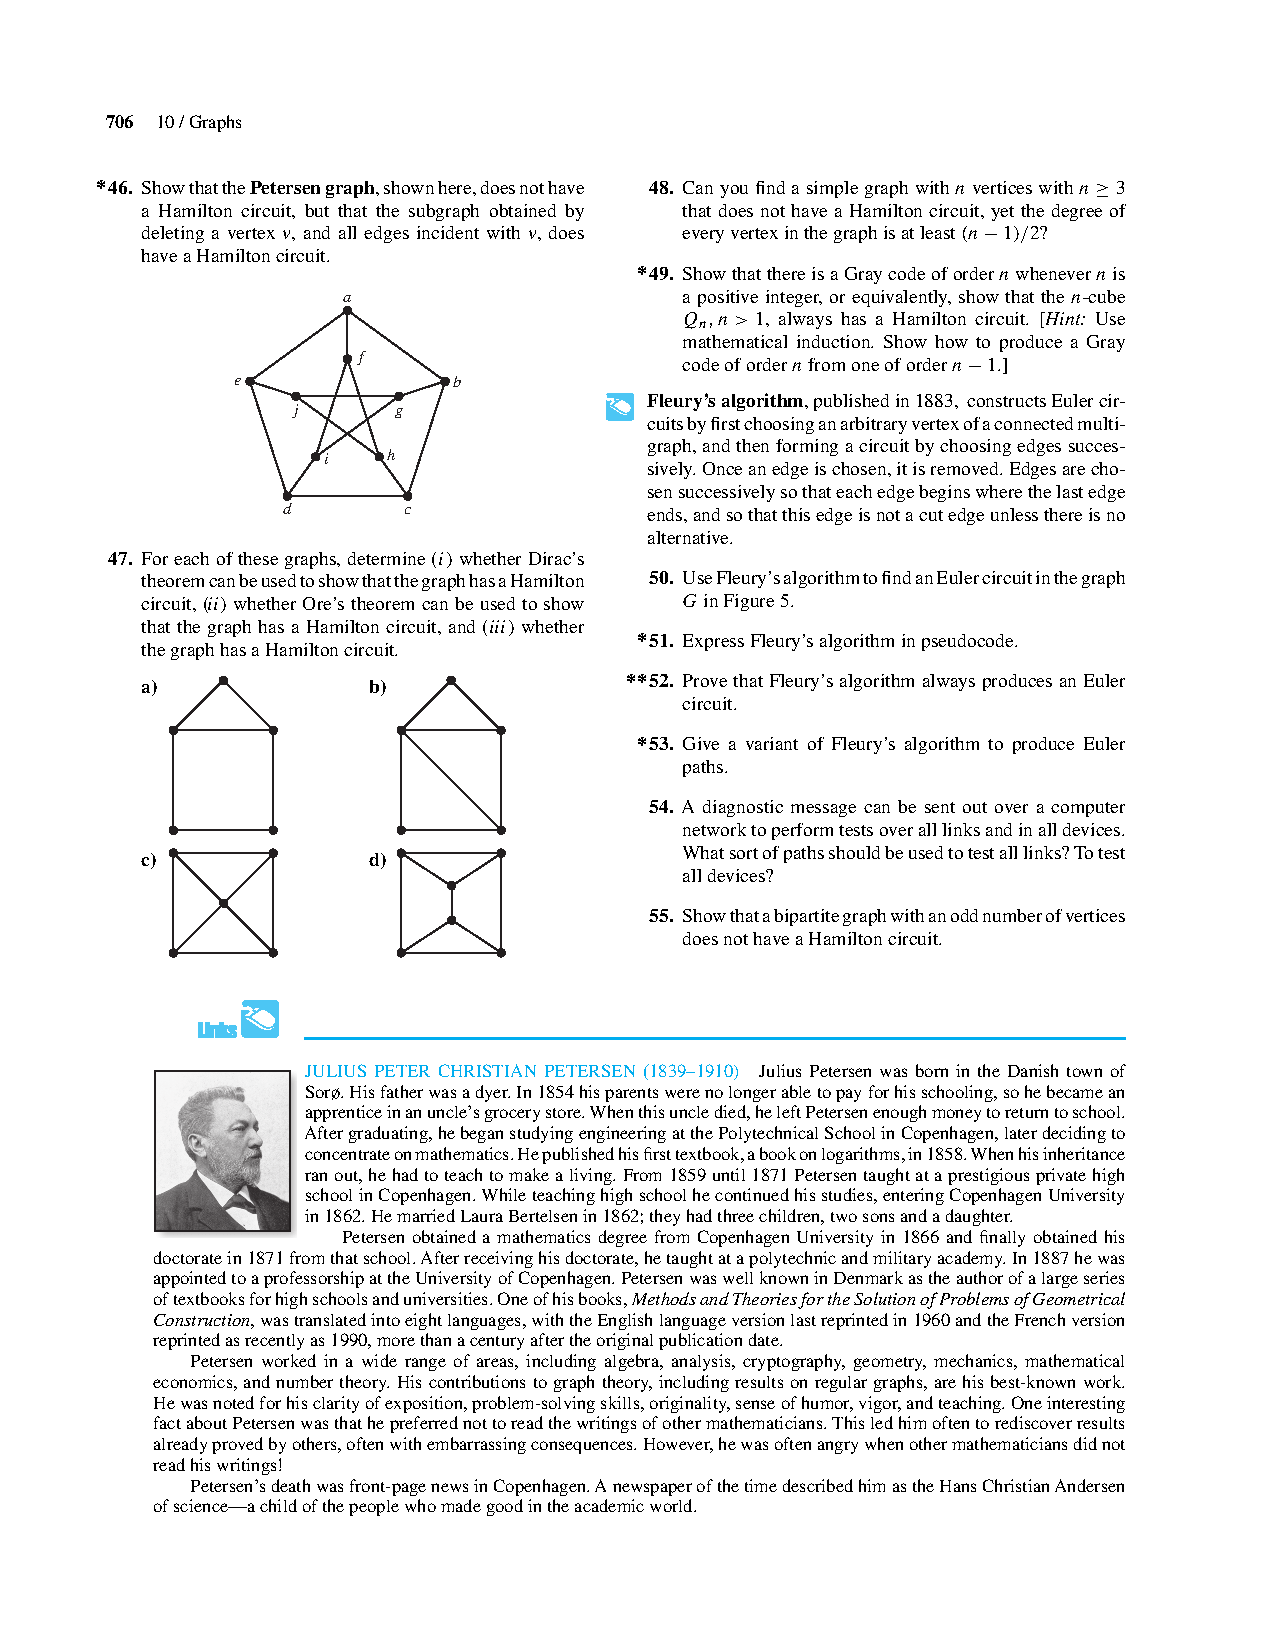
\includegraphics[trim={2.4cm 11.5cm 13cm 11.2cm},clip,width=.45\linewidth]{p706}
\end{frame}

\begin{frame}{Gray codes \footnote{\scriptsize \url{https://en.wikipedia.org/wiki/Gray_code}}}
   \begin{itemize}
        \item Converting the position of a pointer into digital form:
    \end{itemize}
    \centering 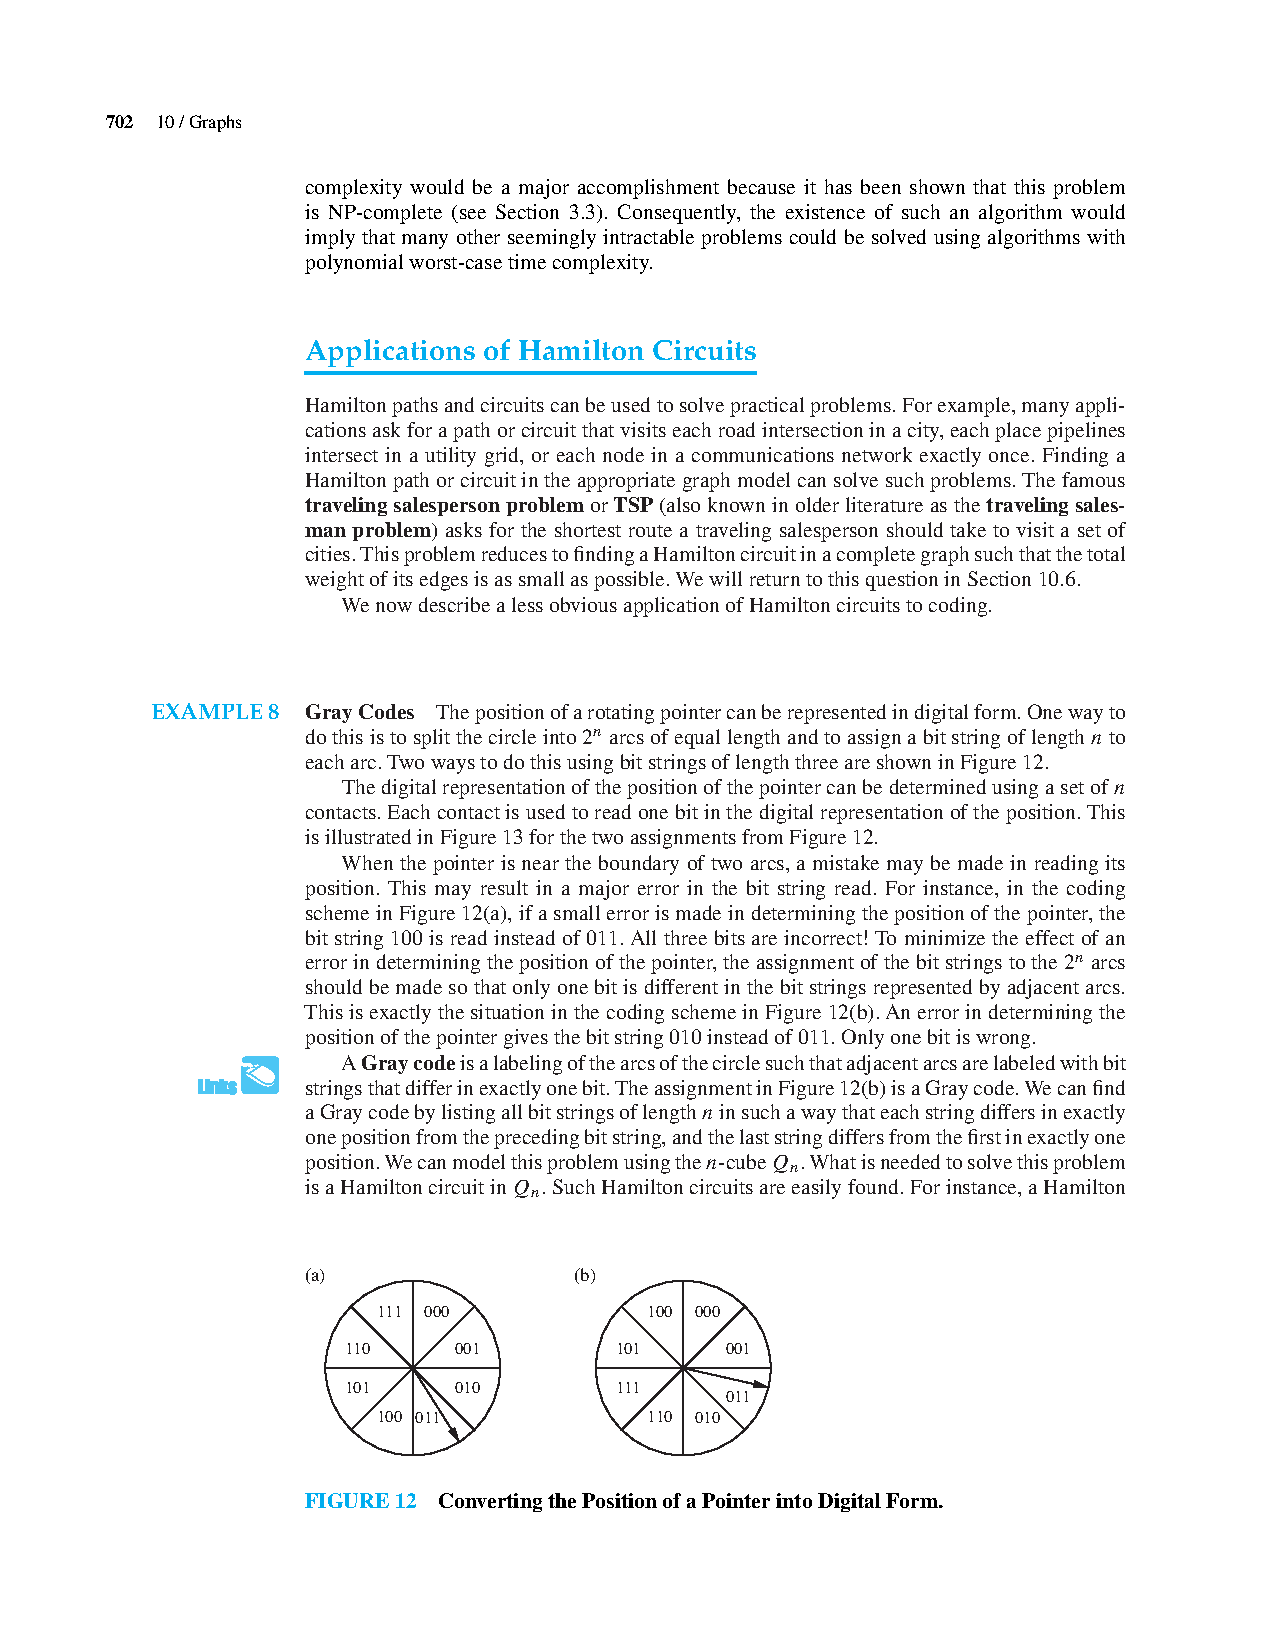
\includegraphics[trim={5cm 3.2cm 8cm 21cm},clip,width=.8\linewidth]{p702}
\end{frame}

\begin{frame}{Gray codes}
   \begin{itemize}
        \item The digital representation of the position of the pointer:
    \end{itemize}
    \centering 
    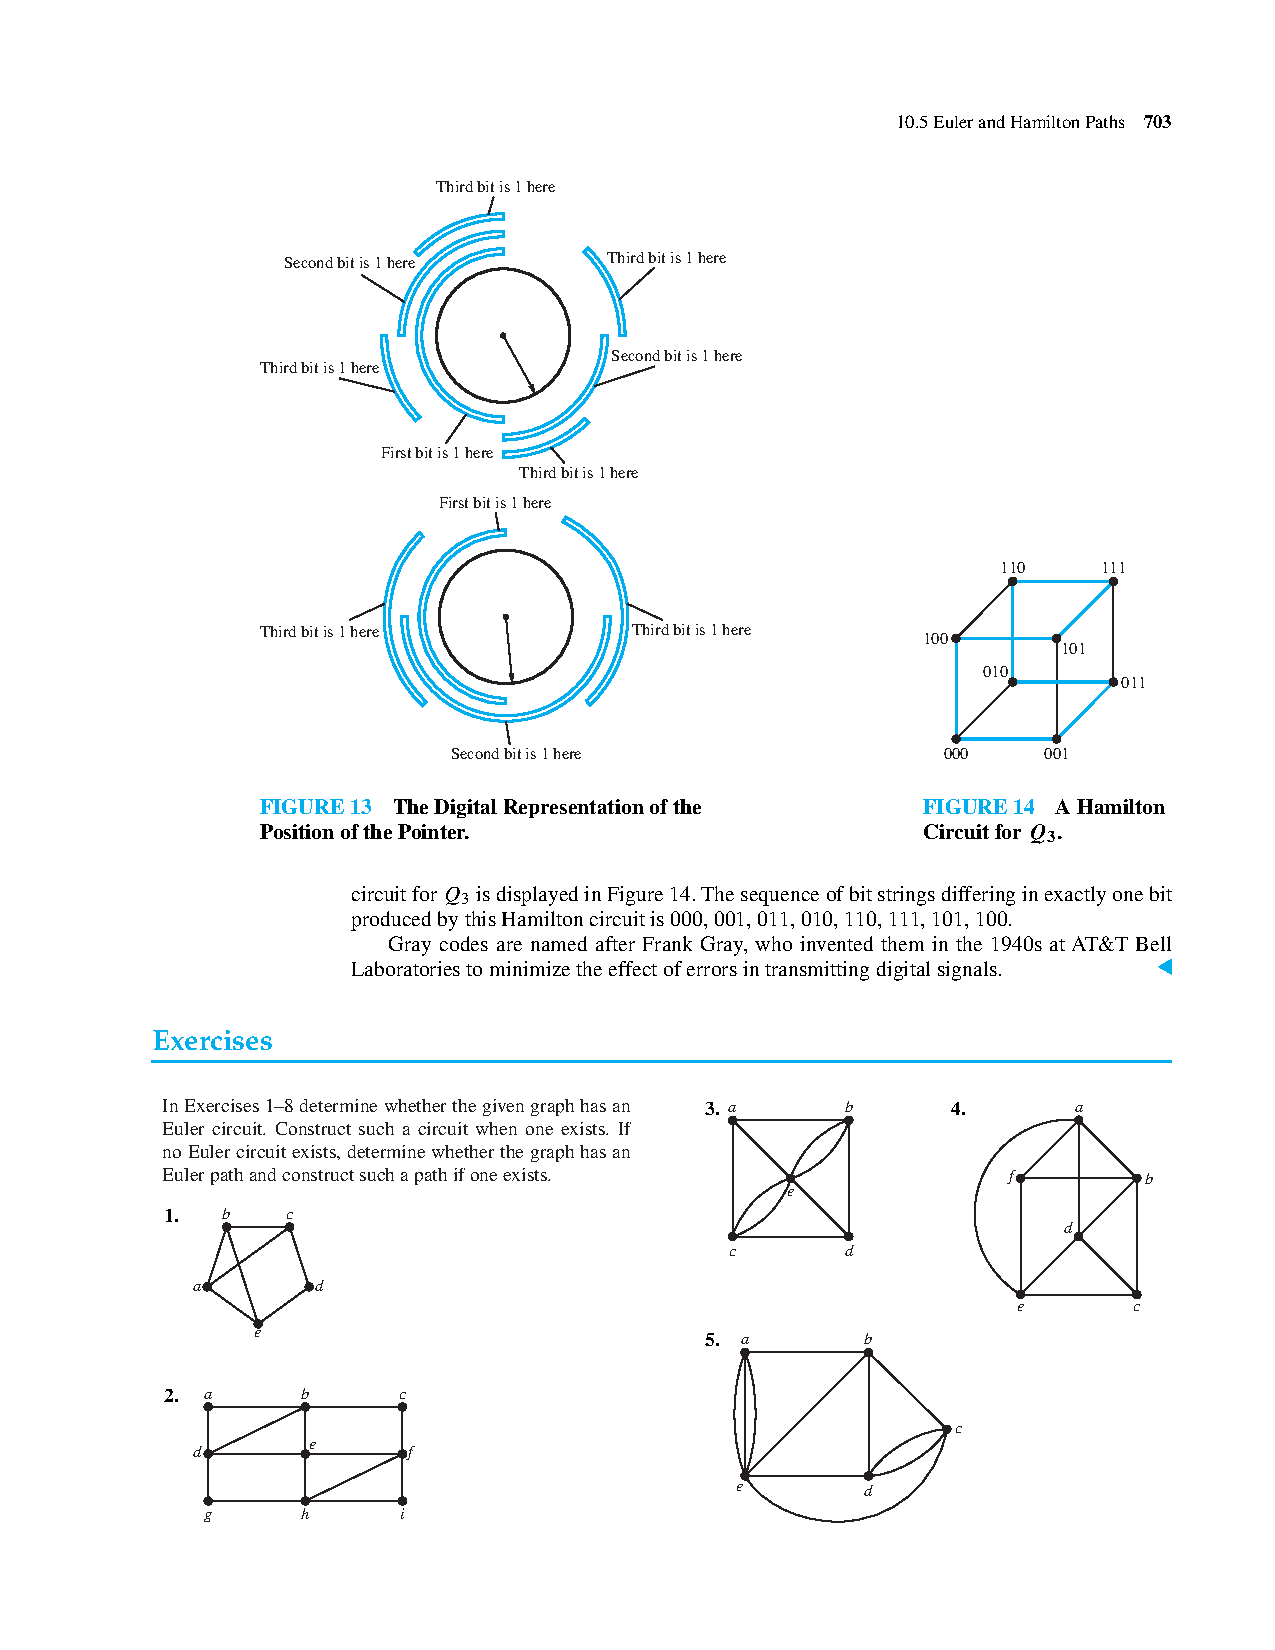
\includegraphics[trim={4.4cm 19.7cm 9cm 3cm},clip,width=.49\linewidth]{p703}
    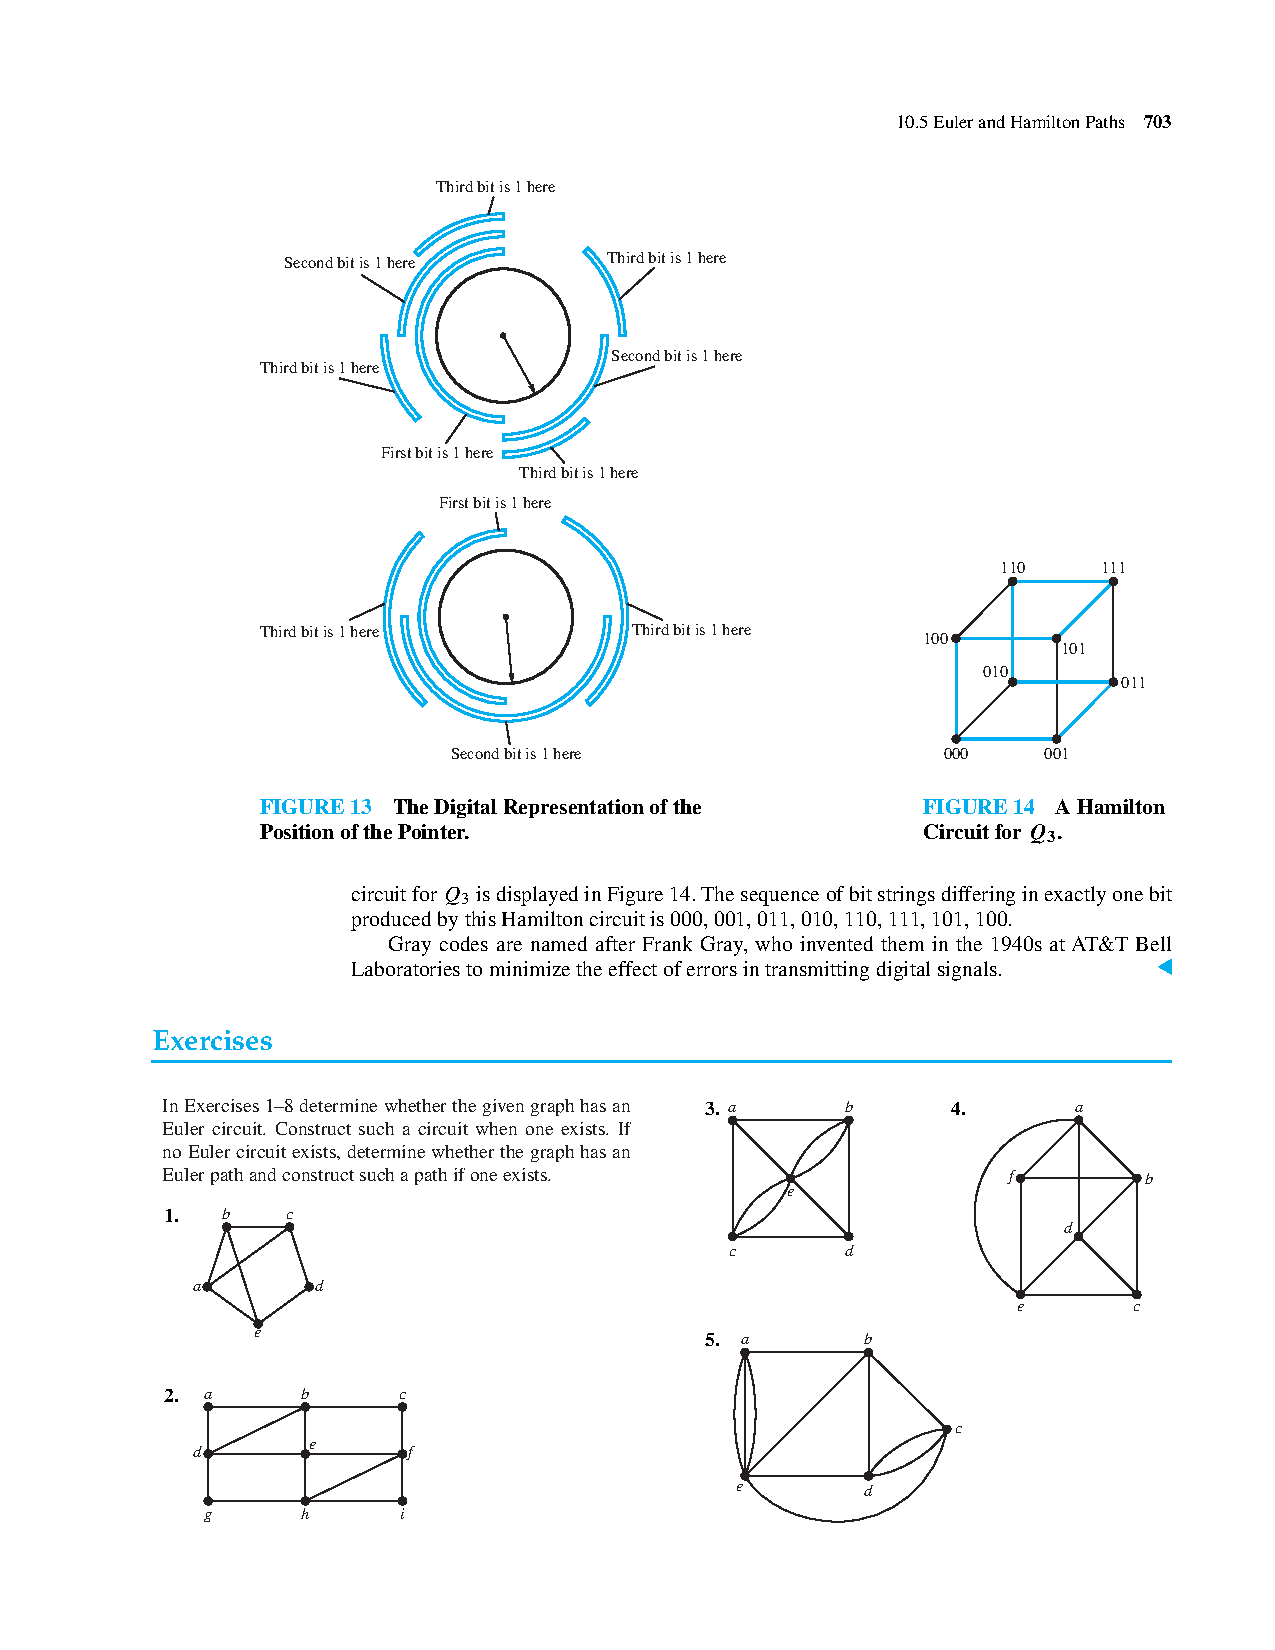
\includegraphics[trim={4.4cm 14.7cm 9cm 8.2cm},clip,width=.49\linewidth]{p703}
\end{frame}

\begin{frame}{Gray codes}
    \centering
    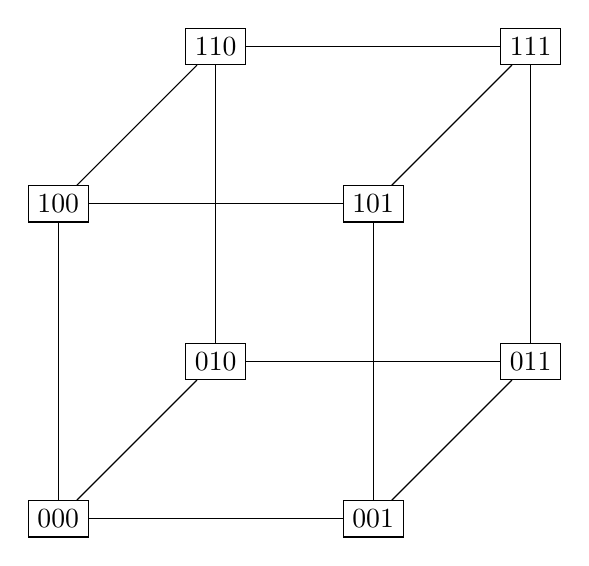
\begin{tikzpicture}
        \node[draw=black] (000) at (0,0) {000};
        \node[draw=black] (001) at (4,0) {001};
        \node[draw=black] (010) at (2,2) {010};
        \node[draw=black] (011) at (6,2) {011};
        \node[draw=black] (100) at (0,4) {100};
        \node[draw=black] (101) at (4,4) {101};
        \node[draw=black] (110) at (2,6) {110};
        \node[draw=black] (111) at (6,6) {111};

        \path [-](000) edge (001);
        \path [-](001) edge (101);
        \path [-](101) edge (100);
        \path [-](100) edge (000);
        \path [-](010) edge (011);
        \path [-](011) edge (111);
        \path [-](111) edge (110);
        \path [-](110) edge (010);
        \path [-](000) edge (010);
        \path [-](001) edge (011);
        \path [-](100) edge (110);
        \path [-](101) edge (111);
    \end{tikzpicture}
\end{frame}

\begin{frame}{Gray codes}
    \centering
    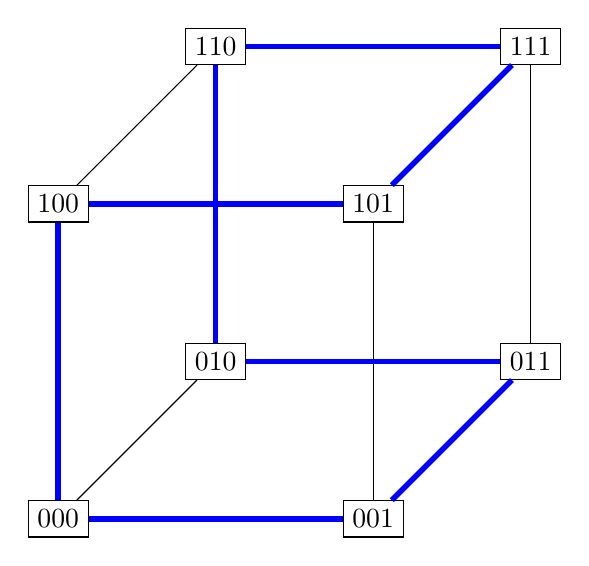
\begin{tikzpicture}
        \node[draw=black] (000) at (0,0) {000};
        \node[draw=black] (001) at (4,0) {001};
        \node[draw=black] (010) at (2,2) {010};
        \node[draw=black] (011) at (6,2) {011};
        \node[draw=black] (100) at (0,4) {100};
        \node[draw=black] (101) at (4,4) {101};
        \node[draw=black] (110) at (2,6) {110};
        \node[draw=black] (111) at (6,6) {111};

        \draw[line width=2pt,color=blue](000) -- (001);
        \draw(001) -- (101);
        \draw[line width=2pt,color=blue](101) -- (100);
        \draw[line width=2pt,color=blue](100) -- (000);
        \draw[line width=2pt,color=blue](010) -- (011);
        \draw(011) -- (111);
        \draw[line width=2pt,color=blue](111) -- (110);
        \draw[line width=2pt,color=blue](110) -- (010);
        \draw(000) -- (010);
        \draw[line width=2pt,color=blue](001) -- (011);
        \draw(100) -- (110);
        \draw[line width=2pt,color=blue](101) -- (111);
    \end{tikzpicture}
\end{frame}

\section{Vertex Coloring}

\begin{frame}{Vertex Coloring}
    \begin{itemize}
        \item The chromatic number of a graph  is the smallest number of colors needed to color the vertices so that no two adjacent vertices share the same color.
        \item Hardness: A very hard problem(an NP-Complete problem).
    \end{itemize}
\end{frame}

\begin{frame}{Vertex Coloring}
    \centering
    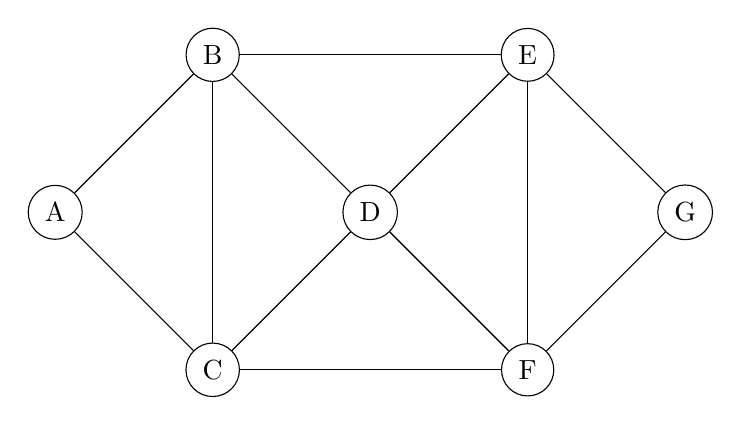
\begin{tikzpicture}
        \node[shape=circle,draw=black] (A) at (0,2) {A};
        \node[shape=circle,draw=black] (B) at (2,4) {B};
        \node[shape=circle,draw=black] (C) at (2,0) {C};
        \node[shape=circle,draw=black] (D) at (4,2) {D};
        \node[shape=circle,draw=black] (F) at (6,0) {F};
        \node[shape=circle,draw=black] (E) at (6,4) {E};
        \node[shape=circle,draw=black] (G) at (8,2) {G};

        \path [-](A) edge (B);
        \path [-](A) edge (C);
        \path [-](B) edge (C);
        \path [-](B) edge (D);
        \path [-](B) edge (E);
        \path [-](C) edge (D);
        \path [-](D) edge (E);
        \path [-](D) edge (F);
        \path [-](D) edge (F);
        \path [-](C) edge (F);
        \path [-](E) edge (G);   
        \path [-](E) edge (F);   
        \path [-](F) edge (G);   
    \end{tikzpicture}
\end{frame}

\begin{frame}{Vertex Coloring}
    \centering
    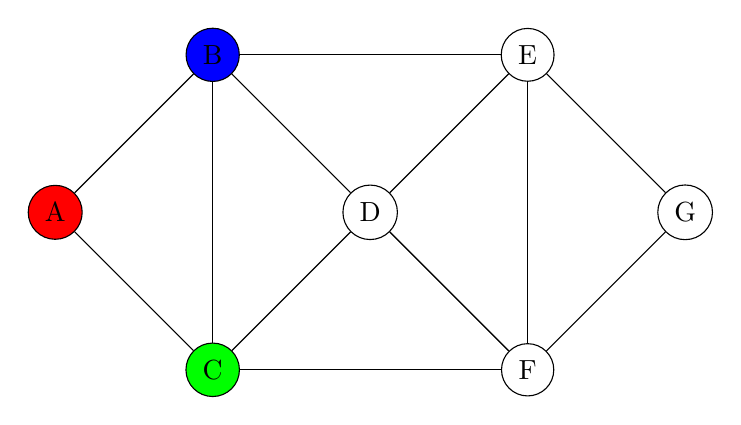
\begin{tikzpicture}
        \node[shape=circle,draw=black,fill=red]   (A) at (0,2) {A};
        \node[shape=circle,draw=black,fill=blue]  (B) at (2,4) {B};
        \node[shape=circle,draw=black,fill=green] (C) at (2,0) {C};
        \node[shape=circle,draw=black] (D) at (4,2) {D};
        \node[shape=circle,draw=black] (F) at (6,0) {F};
        \node[shape=circle,draw=black] (E) at (6,4) {E};
        \node[shape=circle,draw=black] (G) at (8,2) {G};

        \path [-](A) edge (B);
        \path [-](A) edge (C);
        \path [-](B) edge (C);
        \path [-](B) edge (D);
        \path [-](B) edge (E);
        \path [-](C) edge (D);
        \path [-](D) edge (E);
        \path [-](D) edge (F);
        \path [-](D) edge (F);
        \path [-](C) edge (F);
        \path [-](E) edge (G);   
        \path [-](E) edge (F);   
        \path [-](F) edge (G);   
    \end{tikzpicture}
\end{frame}

\begin{frame}{Vertex Coloring}
    \centering
    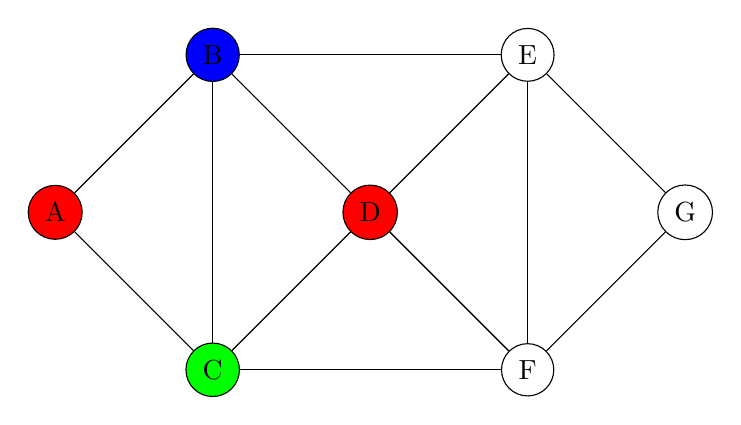
\begin{tikzpicture}
        \node[shape=circle,draw=black,fill=red]   (A) at (0,2) {A};
        \node[shape=circle,draw=black,fill=blue]  (B) at (2,4) {B};
        \node[shape=circle,draw=black,fill=green] (C) at (2,0) {C};
        \node[shape=circle,draw=black,fill=red]   (D) at (4,2) {D};
        \node[shape=circle,draw=black] (F) at (6,0) {F};
        \node[shape=circle,draw=black] (E) at (6,4) {E};
        \node[shape=circle,draw=black] (G) at (8,2) {G};

        \path [-](A) edge (B);
        \path [-](A) edge (C);
        \path [-](B) edge (C);
        \path [-](B) edge (D);
        \path [-](B) edge (E);
        \path [-](C) edge (D);
        \path [-](D) edge (E);
        \path [-](D) edge (F);
        \path [-](D) edge (F);
        \path [-](C) edge (F);
        \path [-](E) edge (G);   
        \path [-](E) edge (F);   
        \path [-](F) edge (G);   
    \end{tikzpicture}
\end{frame}

\begin{frame}{Vertex Coloring}
    \centering
    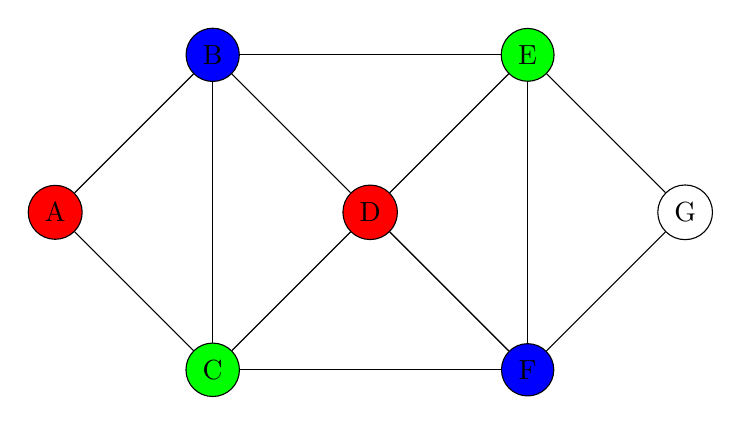
\begin{tikzpicture}
        \node[shape=circle,draw=black,fill=red]   (A) at (0,2) {A};
        \node[shape=circle,draw=black,fill=blue]  (B) at (2,4) {B};
        \node[shape=circle,draw=black,fill=green] (C) at (2,0) {C};
        \node[shape=circle,draw=black,fill=red]   (D) at (4,2) {D};
        \node[shape=circle,draw=black,fill=blue]  (F) at (6,0) {F};
        \node[shape=circle,draw=black,fill=green] (E) at (6,4) {E};
        \node[shape=circle,draw=black] (G) at (8,2) {G};

        \path [-](A) edge (B);
        \path [-](A) edge (C);
        \path [-](B) edge (C);
        \path [-](B) edge (D);
        \path [-](B) edge (E);
        \path [-](C) edge (D);
        \path [-](D) edge (E);
        \path [-](D) edge (F);
        \path [-](D) edge (F);
        \path [-](C) edge (F);
        \path [-](E) edge (G);   
        \path [-](E) edge (F);   
        \path [-](F) edge (G);   
    \end{tikzpicture}
\end{frame}

\begin{frame}{Vertex Coloring}
    \centering
    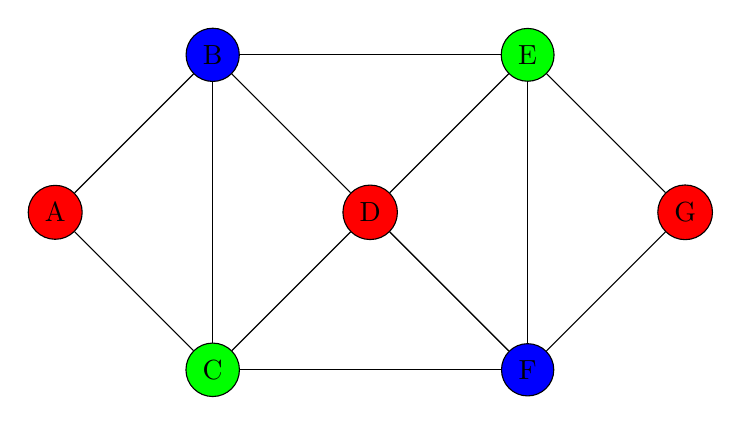
\begin{tikzpicture}
        \node[shape=circle,draw=black,fill=red]   (A) at (0,2) {A};
        \node[shape=circle,draw=black,fill=blue]  (B) at (2,4) {B};
        \node[shape=circle,draw=black,fill=green] (C) at (2,0) {C};
        \node[shape=circle,draw=black,fill=red]   (D) at (4,2) {D};
        \node[shape=circle,draw=black,fill=blue]  (F) at (6,0) {F};
        \node[shape=circle,draw=black,fill=green] (E) at (6,4) {E};
        \node[shape=circle,draw=black,fill=red]   (G) at (8,2) {G};

        \path [-](A) edge (B);
        \path [-](A) edge (C);
        \path [-](B) edge (C);
        \path [-](B) edge (D);
        \path [-](B) edge (E);
        \path [-](C) edge (D);
        \path [-](D) edge (E);
        \path [-](D) edge (F);
        \path [-](D) edge (F);
        \path [-](C) edge (F);
        \path [-](E) edge (G);   
        \path [-](E) edge (F);   
        \path [-](F) edge (G);   
    \end{tikzpicture}
\end{frame}

\begin{frame}{Vertex Coloring}
    \centering
    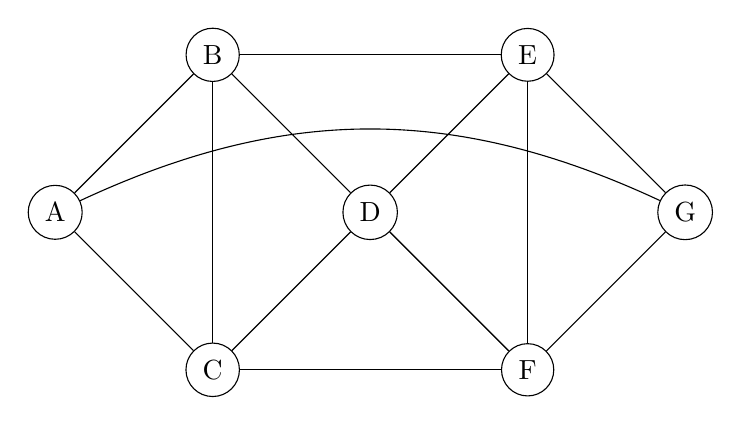
\begin{tikzpicture}
        \node[shape=circle,draw=black] (A) at (0,2) {A};
        \node[shape=circle,draw=black] (B) at (2,4) {B};
        \node[shape=circle,draw=black] (C) at (2,0) {C};
        \node[shape=circle,draw=black] (D) at (4,2) {D};
        \node[shape=circle,draw=black] (F) at (6,0) {F};
        \node[shape=circle,draw=black] (E) at (6,4) {E};
        \node[shape=circle,draw=black] (G) at (8,2) {G};

        \path [-](A) edge (B);
        \path [-](A) edge (C);
        \path [-](B) edge (C);
        \path [-](B) edge (D);
        \path [-](B) edge (E);
        \path [-](C) edge (D);
        \path [-](D) edge (E);
        \path [-](D) edge (F);
        \path [-](D) edge (F);
        \path [-](C) edge (F);
        \path [-](E) edge (G);   
        \path [-](E) edge (F);   
        \path [-](F) edge (G);
        \draw [bend left=25, -](A) to node [auto] {} (G);
    \end{tikzpicture}
\end{frame}

\begin{frame}{Vertex Coloring}
    \centering
    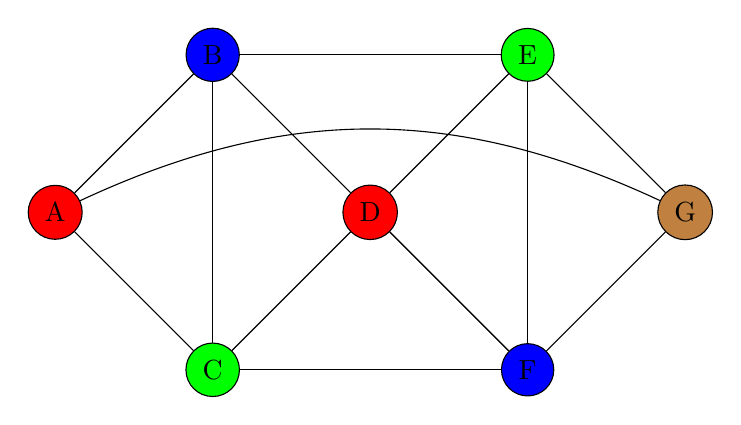
\begin{tikzpicture}
        \node[shape=circle,draw=black,fill=red]  (A) at (0,2) {A};
        \node[shape=circle,draw=black,fill=blue] (B) at (2,4) {B};
        \node[shape=circle,draw=black,fill=green] (C) at (2,0) {C};
        \node[shape=circle,draw=black,fill=red] (D) at (4,2) {D};
        \node[shape=circle,draw=black,fill=blue] (F) at (6,0) {F};
        \node[shape=circle,draw=black,fill=green] (E) at (6,4) {E};
        \node[shape=circle,draw=black,fill=brown] (G) at (8,2) {G};

        \path [-](A) edge (B);
        \path [-](A) edge (C);
        \path [-](B) edge (C);
        \path [-](B) edge (D);
        \path [-](B) edge (E);
        \path [-](C) edge (D);
        \path [-](D) edge (E);
        \path [-](D) edge (F);
        \path [-](D) edge (F);
        \path [-](C) edge (F);
        \path [-](E) edge (G);   
        \path [-](E) edge (F);   
        \path [-](F) edge (G);
        \draw [bend left=25, -](A) to node [auto] {} (G);
    \end{tikzpicture}
\end{frame}

\begin{frame}{Vertex Coloring}
    \centering 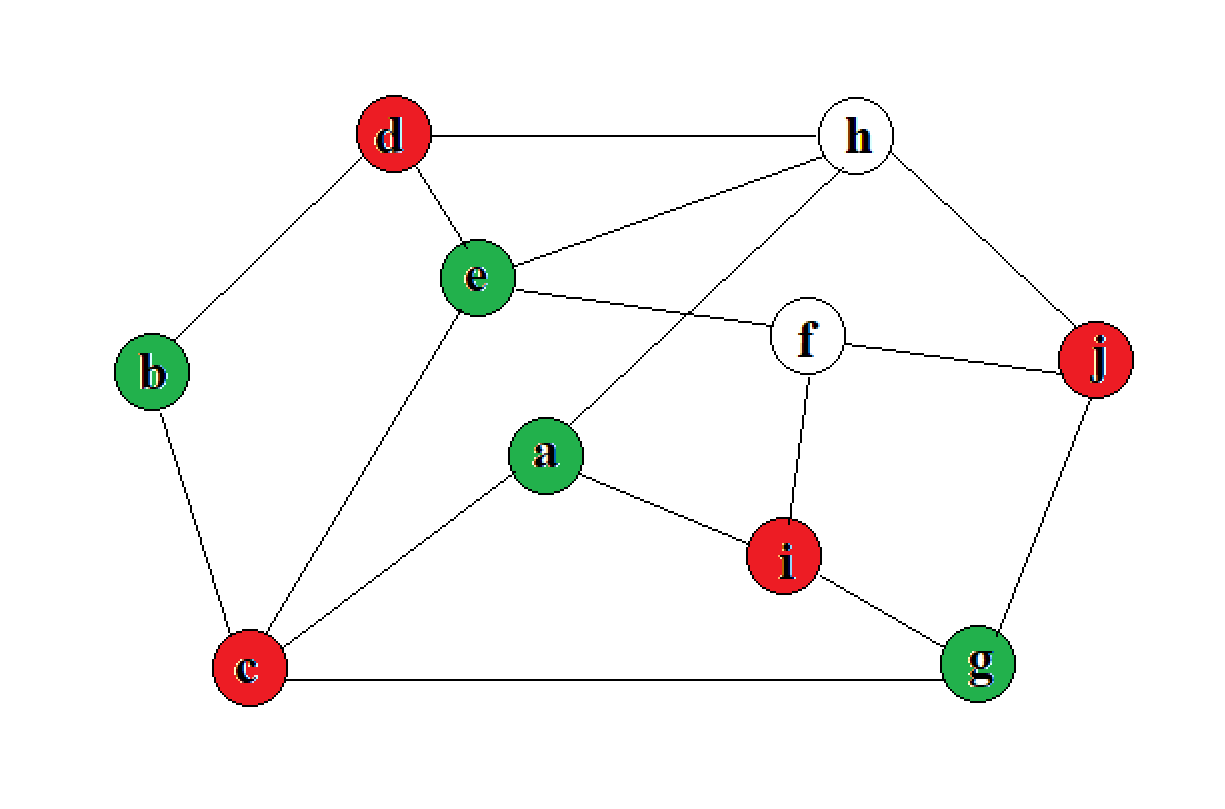
\includegraphics[width=.7\linewidth]{p2.PNG}
\end{frame}

\begin{frame}{Vertex Coloring}
    \centering 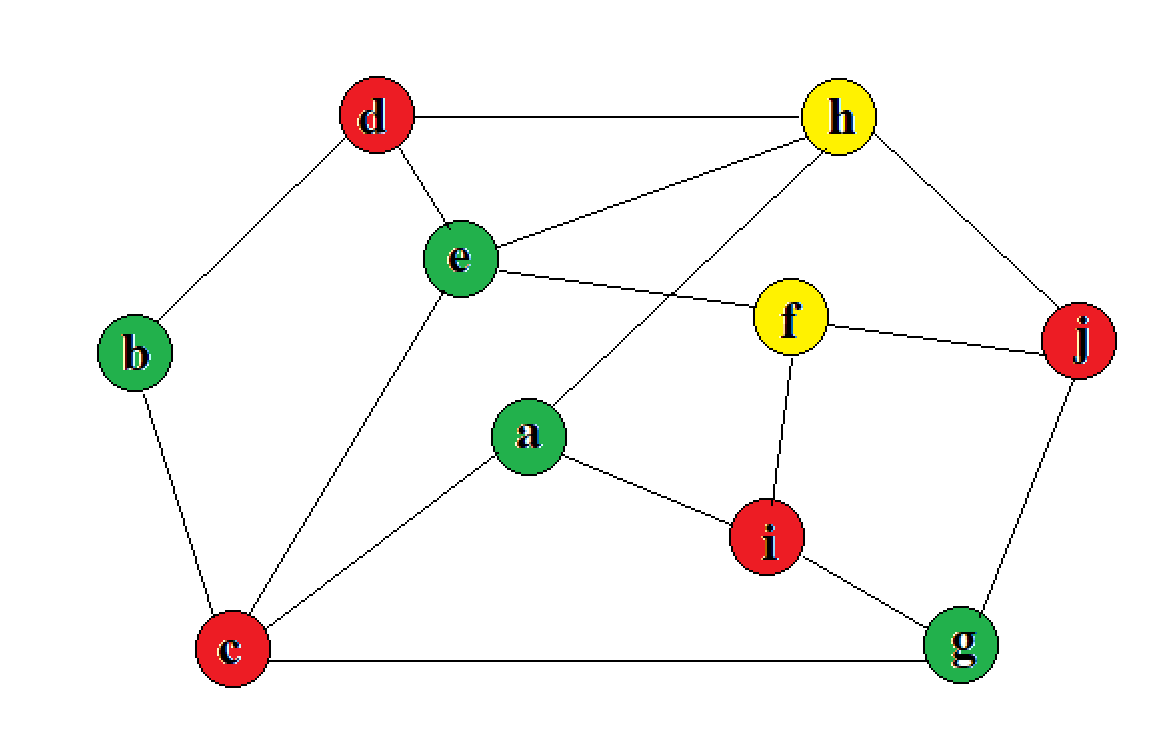
\includegraphics[width=.7\linewidth]{p3.PNG}
\end{frame}

\begin{frame}{Hamiltonian Cycle}
   \begin{itemize}
        \item Complete graphs of $n$ vertices ($K_n$):
    \end{itemize}
    \centering 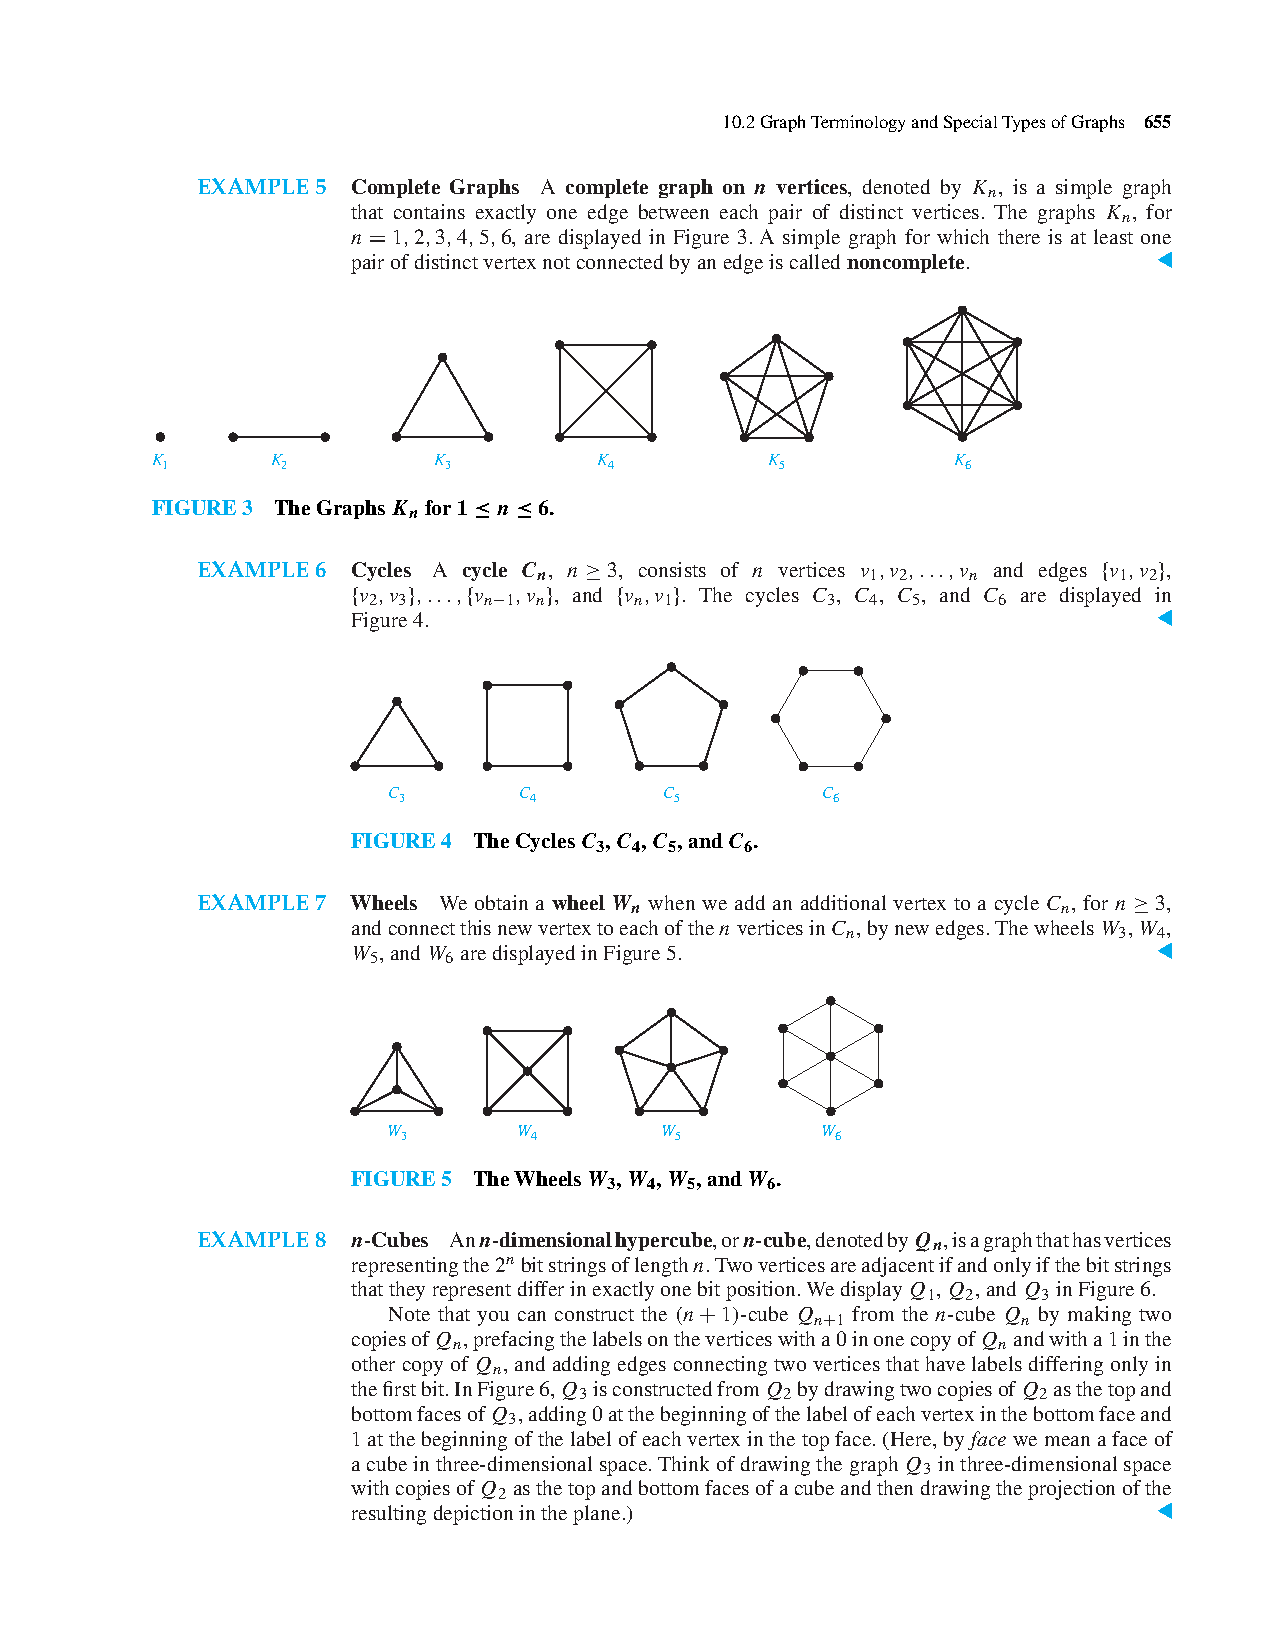
\includegraphics[trim={2cm 20cm 7cm 5cm},clip,width=.9\linewidth]{p655}
\end{frame}

\begin{frame}{Vertex Coloring}
    For certain classes of graphs, we can easily compute the chromatic number. For example, the chromatic number of $K_n$ is $n$, for any $n$. Notice that we have to argue two separate things to establish that this is its chromatic number:
    \begin{itemize}
        \item $K_n$ can be colored with $n$ colors.
        \item $K_n$ cannot be colored with less than $n$ colors.
    \end{itemize}
    For $K_n$, both of these facts are fairly obvious. Assigning a different color to each vertex will always result in a well-formed coloring (though it may be a waste of colors). Since each vertex in $K_n$ is adjacent to every other vertex, no two can share a color. So fewer than $n$ colors can't possibly work.
\end{frame}

\begin{frame}{Vertex Coloring}
    \centering 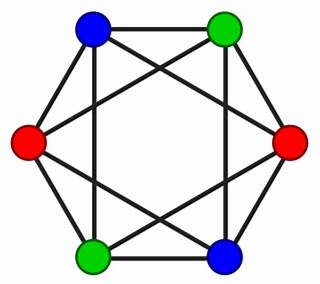
\includegraphics[width=.6\linewidth]{p4.jpg}
\end{frame}

\begin{frame}{Frequency Assignments}
    \begin{itemize}
     \item Television channels 2 through 13 are assigned to stations in Colombia so that no two stations within 150 Km can operate on the same channel. How can the assignment of channels be modeled by graph coloring?
    \end{itemize}
\end{frame}

\begin{frame}{Frequency Assignments}
    \centering 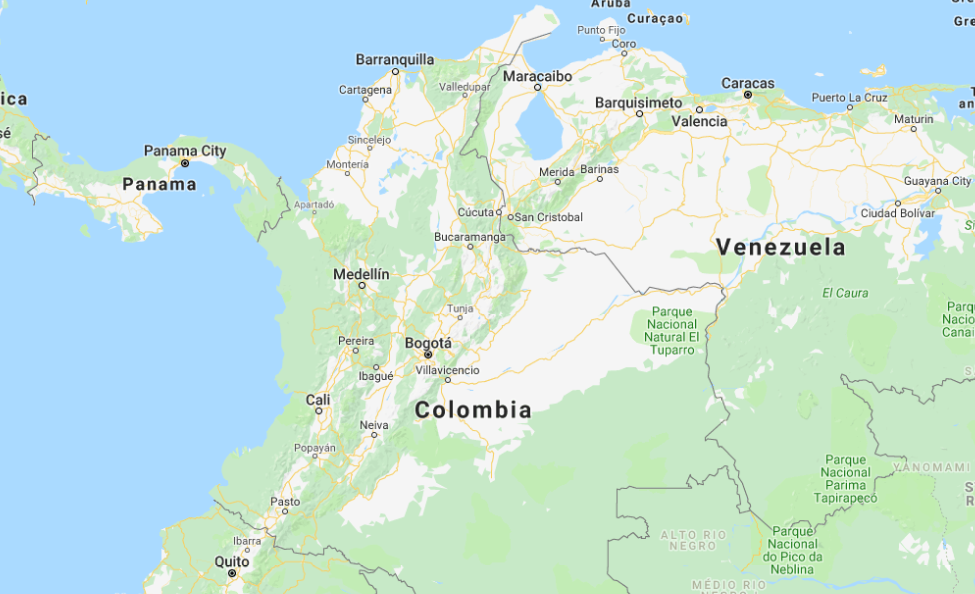
\includegraphics[width=.9\linewidth]{col1.png}
\end{frame}
\begin{frame}{Frequency Assignments}
    \centering 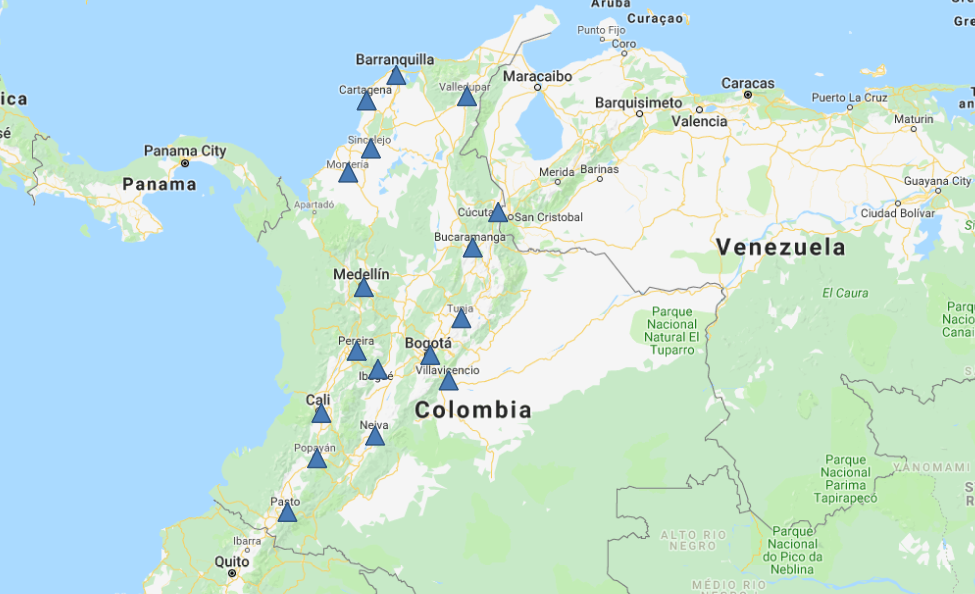
\includegraphics[width=.9\linewidth]{col2.png}
\end{frame}
\begin{frame}{Frequency Assignments}
    \centering 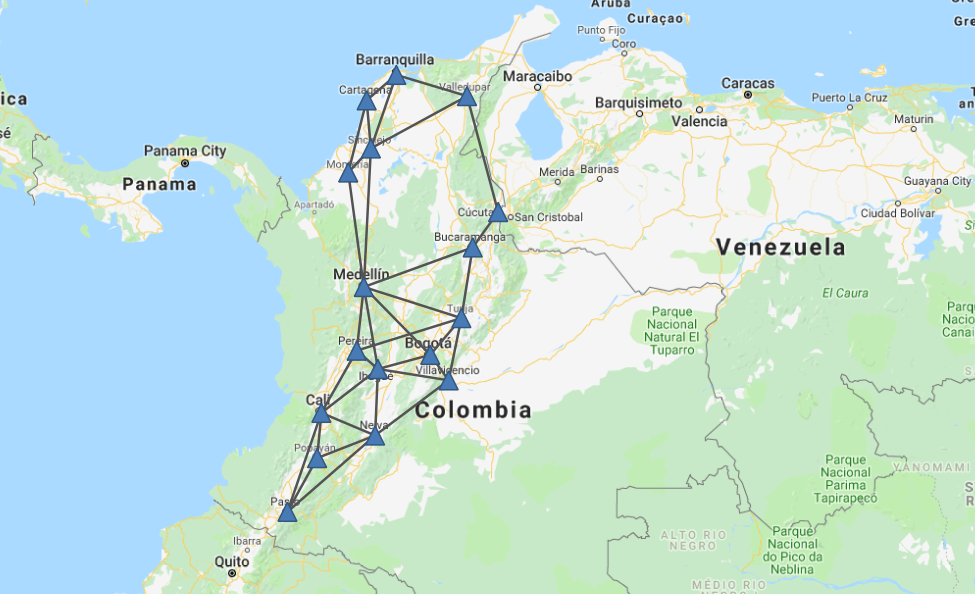
\includegraphics[width=.9\linewidth]{col3.png}
\end{frame}
\begin{frame}{Frequency Assignments}
    \centering 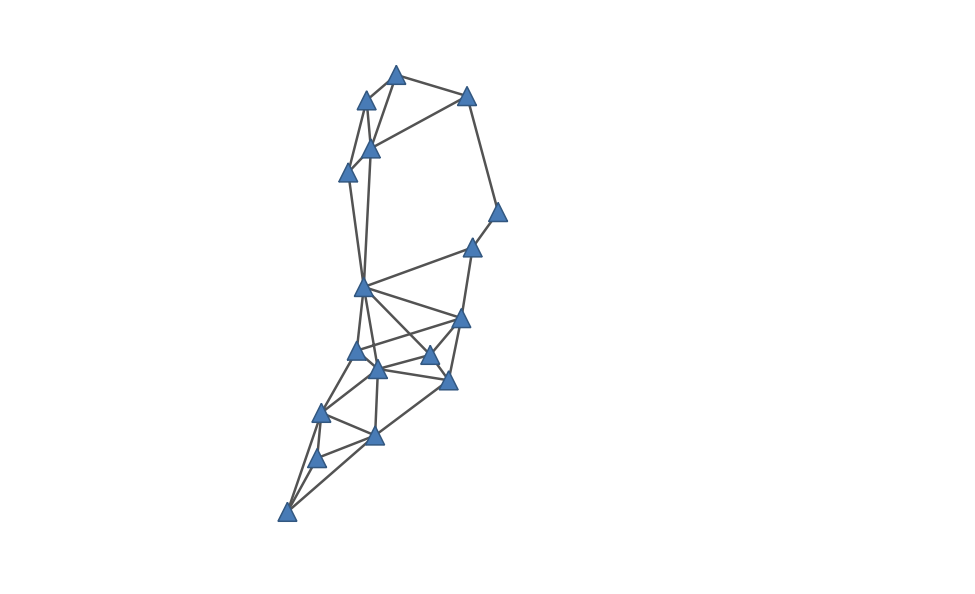
\includegraphics[width=.9\linewidth]{col4.png}
\end{frame}

\begin{frame}{Frequency Assignments}
    \begin{itemize}
        \item Television channels 2 through 13 are assigned to stations in Colombia so that no two stations within 150 Km can operate on the same channel. How can the assignment of channels be modeled by graph coloring?
        \item Construct a graph by assigning a vertex to each station. Two vertices are connected by an edge if they are located within 150 Km of each other. An assignment of channels corresponds to a coloring of the graph, where each color represents a different channel.
    \end{itemize}
\end{frame}

\section{Bipartite graph}

\begin{frame}{Bipartite graph}
    \begin{itemize}
        \item A bipartite graph, also called a bigraph, is a set of graph vertices decomposed into two disjoint sets such that no two graph vertices within the same set are adjacent.
        \item Bipartite graphs are equivalent to two-colorable graphs. 
        \item All acyclic graphs are bipartite. 
        \item A cyclic graph is bipartite iff all its cycles are of even length
    \end{itemize}
\end{frame}

\begin{frame}{Bipartite graph}
    \centering 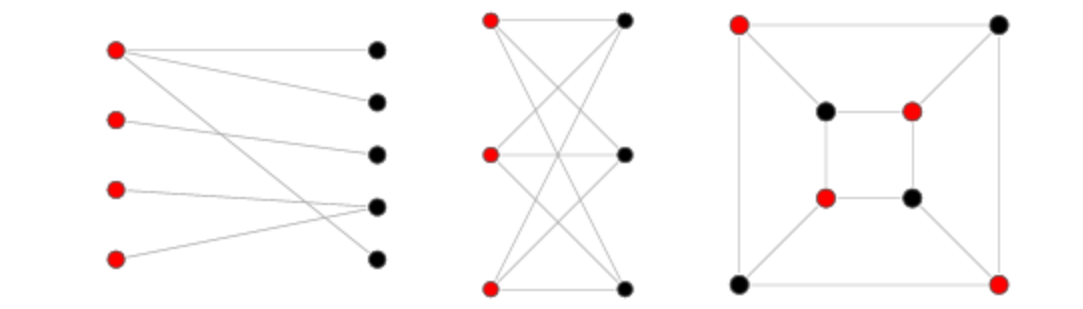
\includegraphics[width=.7\linewidth]{p5.PNG}
\end{frame}

\section{Perfect matching}

\begin{frame}{Perfect matching}
A perfect matching of a graph is a matching (i.e., an independent edge set) in which every vertex of the graph is incident to exactly one edge of the matching. 
\\A perfect matching is therefore a matching containing $\frac{n}{2}$ edges (the largest possible), meaning perfect matchings are only possible on graphs with an even number of vertices.
\end{frame}

\begin{frame}{Perfect matching}
 Hall’s Theorem: Let G = (X,Y ) be a bipartite graph. Then X has a perfect macthing into Y if and only if for all $T \subseteq X$, the inequality $|T| \leq |N(T)|$ holds. Where N(T) is the set of all neighbors of the vertices in T. In other words, $y \in  Y$ is an element of N(T) if and only if there is a vertex $x \in  T$ so that xy is an edge.
\end{frame}

\begin{frame}{Perfect matching}
    \begin{flushleft}
        You are given two bipartite graph G and H below. For each graph determine whether it has a perfect matching. Justify your answer, either by listing the edges that are in the matching or use Hall's Theorem to show that the graph does not have a perfect matching.
    \end{flushleft}
    \centering 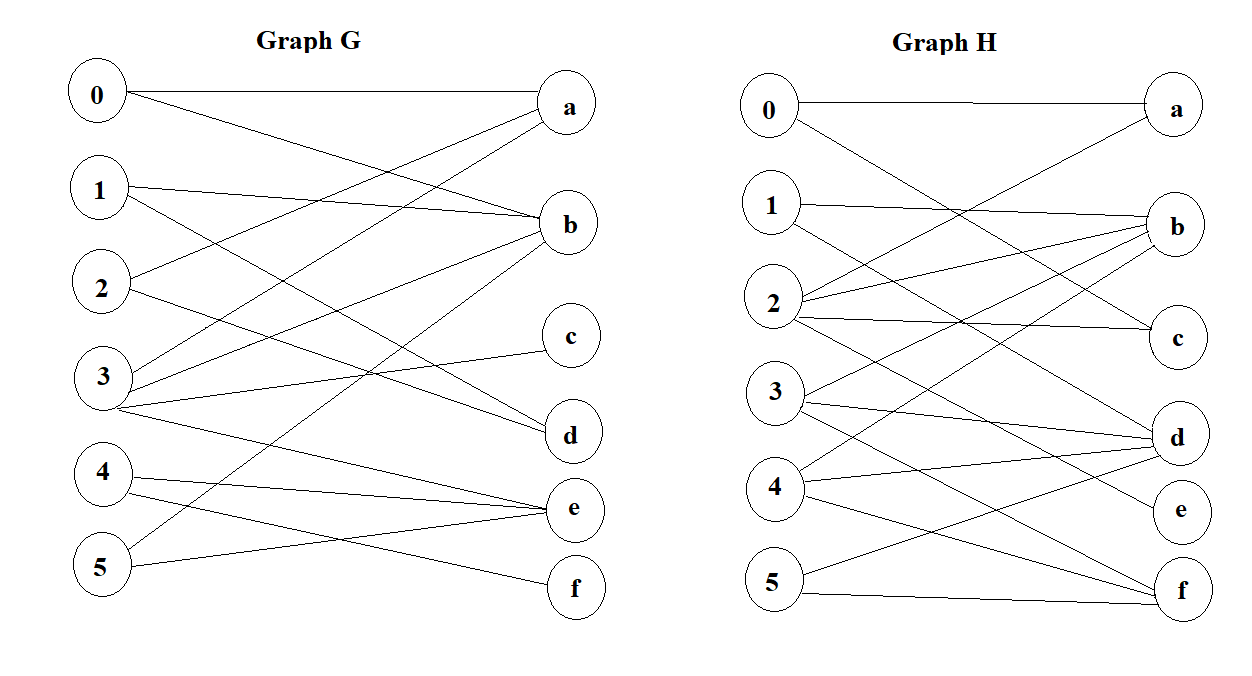
\includegraphics[width=.7\linewidth]{p6.jpg}
\end{frame}

\begin{frame}{Perfect matching}
    \centering 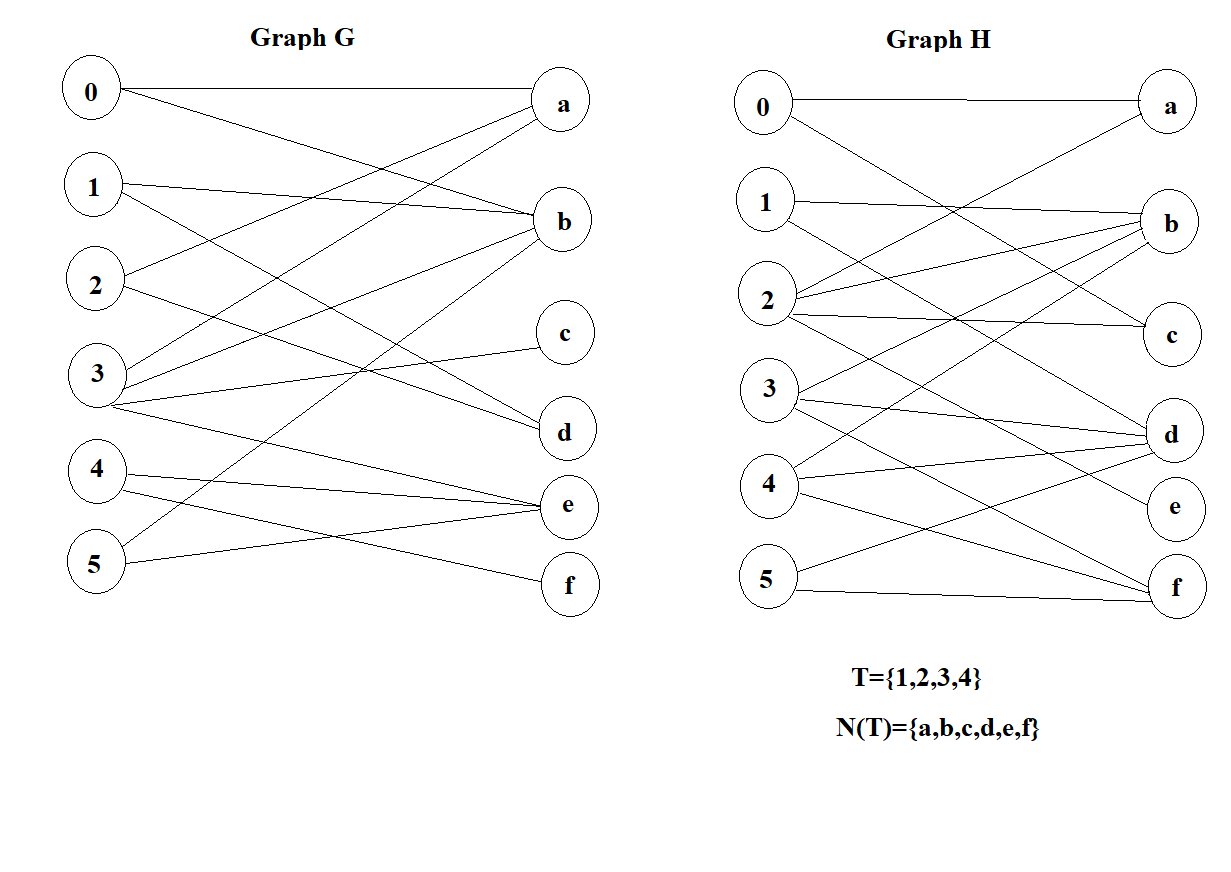
\includegraphics[width=.7\linewidth]{p7.PNG}
\end{frame}

\section*{Reference}

\begin{frame}{Reference}
    \begin{itemize}
        \item Discrete Mathematics and Its Applications. Rosen, K.H. 2012. McGraw-Hill. \\
        Chapter 10: Graphs. \\
        Section 10.5: Euler and Hamilton Paths. \\
        Section 10.8: Graph Coloring.
    \end{itemize}
\end{frame}

\end{document}
